%==============================================================
\chapter{IMPLEMENTATION AND EXPERIMENTAL RESULTS}
\label{ch:impl}
%==============================================================

\section{Experimental Setup}
\label{sec:setup}

\tabref{tab:setup} lists the machines and environments used for development, training, evaluation and deployment.

\begin{table}[htbp]
\caption{Experimental and deployment environments}
\label{tab:setup}
\centering\tablefont
\begin{tabularx}{\textwidth}{|L{3.0cm}|Y|L{3.5cm}|}
\hline\rowhead
\thead{Machine} & \thead{Configuration} & \thead{Used for}\\ \hline
Development laptop & Intel Core i7-14650HX (24 threads), Windows 11, Python 3.14 virtual environment with CPU PyTorch & Evaluation, benchmarks (with 4 threads to mimic the Pi), tests, demo world\\ \hline
Training environment & Same laptop, NVIDIA RTX 4060 (8\,GB), separate Python 3.11 environment with CUDA PyTorch, Ultralytics, timm & Training the scene classifier, YOLO heads and slim heads\\ \hline
Raspberry~Pi~5 unit & 8\,GB, Raspberry~Pi~OS Trixie, Camera Module 3, Active Cooler; SENTRIX as a systemd user service in clip mode (ONNX, 320\,px object stage, fast lane, \code{buffalo\_s} faces) & Deployment in the demo room, on-device benchmarks, room calibration\\ \hline
Portal & Render web service (0.5 CPU, 512\,MB, Singapore) with a 1\,GB persistent disk, built from \code{deploy/portal/Dockerfile} & Accounts, owner prompts, Desk, tunnel for the demonstration\\ \hline
Test-mode demo world & \code{tools/demo\_reset.py} and \code{tools/demo\_run.py}: Portal and device on the laptop, a demo-reel camera playing recorded clips, every live switch forced off & End-to-end and browser tests, screenshots, rehearsals\\ \hline
\end{tabularx}
\end{table}

\paragraph{Evaluation tools.} Every measurement in this chapter was produced by a tool in the repository, and the report it wrote is committed under \code{training/runs/}:
\code{tools/eval\_custom\_frames.py} (per-image scores), \code{tools/replay\_custom\_videos.py} (the labelled videos through \code{Pipeline.process} at 6\,Hz with true timestamps, tick or clip mode, with the videos' own soundtracks), \code{tools/replay\_decisions.py} (re-decides a recorded live event log under the current rules), \code{tools/bench\_live.py} and \code{tools/bench\_clip.py} (the live loop with a video file as a 30\,fps camera), \code{tools/reid\_eval.py} (body re-identification pairs), \code{tools/eval\_models.py} (every vision model on every dataset it applies to), \code{tools/calibrate\_room.py} (per-room thresholds from the device's own log), and \code{tools/gate\_report.py} (the release gates). All of them run inside the side-effect-free harness described in Section~\ref{sec:investigative}, and all refuse the test video \code{wa02} unless it is evaluated as part of the full set.

%--------------------------------------------------------------
\section{Experimental Analysis}

\subsection{Data}
\label{sec:data}

\paragraph{Data sources.} Three kinds of data were used.
\begin{enumerate}
\item \textbf{Public corpora} for the first (v3) models: RWF-2000 violence clips \cite{cheng2021rwf}, Roboflow weapon and fire/smoke image sets, and AudioSet clips \cite{gemmeke2017audioset} for the first sound model. An audit of their splits (\code{tools/audit\_splits.py}) found that 52.7\,\% of the RWF-2000 validation rows shared source videos with training and that 12.2\,\% of the weapon and 20.0\,\% of the fire validation images were near-duplicates of training images, so their published scores are optimistic. They were used only for pre-training and rehearsal.
\item \textbf{The SENTRIX custom dataset}: ten videos recorded by the team---a bedroom with replica handguns and aerosol flame jets, and a corridor filmed by CCTV with a long stick, an assault and a bicycle theft. From them, 765 frames were hand-reviewed and labelled into five classes (\tabref{tab:dataset}); five more videos added in November bring the set to 977 frames (\tabref{tab:dataset-new}).
\item \textbf{Deployment logs}: the demonstration Pi's own event log in the demo room (about 12 hours, no threat present, and later its whole log from 23 October to 19 November) and the event log of the first live laptop session (18.3 minutes). These are used for calibration and regression, never for training.
\end{enumerate}

\begin{table}[htbp]
\caption{The custom dataset as used for the v4 models (the first ten videos; frames per class and split; splits by source video)}
\label{tab:dataset}
\centering\tablefont
\begin{tabular}{|l|c|c|c|c|}
\hline\rowhead
\thead{Class} & \thead{Train} & \thead{Validation} & \thead{Test} & \thead{Total}\\ \hline
Normal & 373 & 23 & 67 & 463\\ \hline
Fire & 11 & 6 & 0 & 17\\ \hline
Weapon (handgun, stick) & 144 & 55 & 26 & 225\\ \hline
Assault & 43 & 0 & 0 & 43\\ \hline
Robbery & 17 & 0 & 0 & 17\\ \hline
\textbf{Videos} & vid02, vid03, vid05, vid06, vid07, wa01, wa03 & gun, vid04 & wa02 & 10\\ \hline
\end{tabular}
\end{table}

\paragraph{Five videos added in November.} On 18 November 2026 the team added five videos: four masked-intruder scenes in the bedroom (a handgun pointed at a seated person, a knife attack, a beating with a metal flask, and a theft from the wardrobes) and one ordinary scene in a second room (\tabref{tab:dataset-new}). They were extracted with the original sampling rules and reviewed segment by segment, and they joined the training split; no video was held out. Grounding DINO proposed 27 boxes for them; 13 were kept after visual checks (7 pistol, 6 knife) and 14 rejected (a phone, a monitor). The dataset now holds 977 frames from fifteen videos and 180 checked boxes.

\begin{table}[htbp]
\caption{The five videos added on 18 November 2026 (all in the training split)}
\label{tab:dataset-new}
\centering\tablefont
\begin{tabularx}{\textwidth}{|l|Y|c|}
\hline\rowhead
\thead{Video} & \thead{Content} & \thead{Frames kept}\\ \hline
mmtheft & Masked intruder searches the shoe rack and wardrobes and leaves with items & 99 (robbery 62)\\ \hline
mmassault & Masked intruder strikes a person on the bed with a metal flask & 26 (assault 13)\\ \hline
mmgun & Handgun pointed at a seated person; a phone snatched at gunpoint & 23 (weapon 19)\\ \hline
mmknife & Knife attack on a person lying on the bed & 35 (weapon 28)\\ \hline
nvroom2 & Second room: three people, ordinary activity & 29 (normal)\\ \hline
\textbf{Total} & normal 90, weapon 47, assault 13, robbery 62 & \textbf{212}\\ \hline
\end{tabularx}
\end{table}

\paragraph{Cleaning and pruning.} Frames were sampled at 3--8\,fps, near-duplicates were dropped with a perceptual hash, and every kept frame was reviewed by a person. For video replay a label \emph{timeline} was built from every sampled frame: a kept frame carries its reviewed label; a dropped near-duplicate inherits its kept twin's label only if the twin is within 1\,s (a perceptual hash barely registers a flame jet, so a ``duplicate'' 5\,s away can differ in exactly the object that decides the label), otherwise it keeps its own segment label if that segment was confident ($\geq 0.7$), otherwise it is not scored. A replay tick is scored against the nearest sample within 0.25\,s.

\paragraph{Annotation and feature extraction.} Bounding boxes for the YOLO heads were proposed by Grounding DINO \cite{liu2024groundingdino} but kept only when gated by the reviewed frame label, a held-object check (the box must overlap a person's hands region) and a visual quality check: 167 boxes were kept and 16 rejected. The scene classifier sees each frame resized to 224\,px with ImageNet normalisation; the body embedder sees person crops padded to an aspect ratio of 0.5 and resized to 256$\times$128; the sound tagger sees 4\,s of 16\,kHz mono audio as a log-mel spectrogram. \figref{fig:datapipe} summarises the workflow.

\begin{figure}[htbp]
\centering
\resizebox{\textwidth}{!}{%
\begin{tikzpicture}[node distance=4mm, s/.style={draw, rounded corners=2pt, fill=sxlight, font=\scriptsize, align=center, text width=2.2cm, minimum height=10mm}, a/.style={-{Stealth[length=1.6mm]}, thick}]
\node[s] (v) {15 source videos\\(3 rooms)};
\node[s, right=of v] (f) {Frame sampling\\3--8\,fps};
\node[s, right=of f] (h) {Perceptual-hash\\de-duplication};
\node[s, right=of h] (r) {Human review:\\977 labelled frames};
\node[s, right=of r] (t) {Label timeline\\(1\,s rule)};
\node[s, below=6mm of r] (b) {Grounding DINO boxes,\\label-gated + QC\\(180 kept, 30 rejected)};
\node[s, below=6mm of t] (sp) {Split by video:\\7 train, 2 val, 1 test};
\node[s, left=of b] (tr) {Training: DINOv2 head,\\YOLO11n heads};
\node[s, left=of tr] (cv) {LOVO selection on\\9 videos, OOF\\temperature, thresholds};
\node[s, left=of cv] (te) {Confirm on val,\\report test once};
\draw[a] (v) -- (f); \draw[a] (f) -- (h); \draw[a] (h) -- (r); \draw[a] (r) -- (t); \draw[a] (t) -- (sp); \draw[a] (r) -- (b); \draw[a] (sp) -- (b); \draw[a] (b) -- (tr); \draw[a] (tr) -- (cv); \draw[a] (cv) -- (te);
\end{tikzpicture}}
\caption{Data workflow from the team's videos to selected models}
\label{fig:datapipe}
\end{figure}

\paragraph{Deployment-room data.} Because no model can be validated for a room it has never seen, the product records its own training data: the device administrator (or the owner, with a fresh password check) starts a recording on the dashboard; the device writes the camera's raw frames as a constant-frame-rate MJPEG video with the microphone's 16\,kHz audio muxed in, plus a JSON sidecar; recordings stop after 10 minutes, keep 2\,GB of disk free for evidence, are deleted after 14 days and can only be downloaded on the home network. Everyone filmed must consent.

\subsection{Performance Parameters}
\label{sec:perf-params}
\paragraph{Classification measures (per image or per tick).} Accuracy; \emph{macro-F1}, averaged only over the classes present in the split's ground truth (the test split has two, so a perfect model scores 1.0); threat recall and false-positive rate (normal versus any threat); and the area under the ROC curve (AUROC) \cite{fawcett2006roc} of a class probability against normal frames, which is threshold-free.

\paragraph{Alarm measures (per video replay).} An \emph{episode} is a contiguous run of ground-truth threat; it is detected at level $L$ if the matching class is committed at level $\geq L$ between its start and 1\,s after its end. A \emph{false onset} is a commit to level $\geq L$ on normal footage more than 1\,s from any episode. For $k$ false onsets in $T$ hours of normal footage the rate is $k/T$ with an exact Poisson 95\,\% interval; for $k=0$ the upper bound is
\begin{equation}
\lambda_{95} = \frac{-\ln(0.025)}{T} = \frac{3.689}{T}\ \text{per hour},
\end{equation}
so 3.7 minutes of normal footage can only show a rate below about 60 per hour. Recall per level carries a Clopper--Pearson interval \cite{clopper1934}. Latency is measured from the episode's start to the commit (median and 95th percentile).

\paragraph{Quality-of-service measures.} Preview frame rate (video fps), AI decision rate (Hz), tick latency and frame age (p50/p95), per-stage latency; on the Pi, clip compute time, the share of clips dropped because the previous clip was still running, and the age of a decision; for the Portal, the time from a scene to a pending request, from approval to dispatch, and the frame rate of remote video.

%--------------------------------------------------------------
\section{Working of the Project}

\subsection{Procedural Workflow}
\label{sec:workflow}
\figref{fig:workflow} shows the complete workflow of the product from installation to a closed incident. It has four phases.

\begin{figure}[htbp]
\centering
\resizebox{\textwidth}{!}{%
\begin{tikzpicture}[node distance=3.5mm, s/.style={draw, rounded corners=2pt, fill=sxlight, font=\scriptsize, align=center, text width=2.6cm, minimum height=11mm}, ph/.style={font=\scriptsize\bfseries, text=sxblue}, a/.style={-{Stealth[length=1.6mm]}, thick}]
\node[s] (p1) {Company provisions device:\\id, serial, claim code};
\node[s, below=of p1] (p2) {Customer activates,\\completes 7-step\\onboarding};
\node[s, below=of p2] (p3) {Device claimed; faces\\enrolled from the\\device camera};
\node[s, right=8mm of p1] (m1) {Capture frames;\\newest frame or\\4\,s clip analysed};
\node[s, below=of m1] (m2) {Models vote; evidence\\confirmed; TCI and\\level committed};
\node[s, below=of m2] (m3) {Level 3: snapshot,\\encrypted evidence,\\assistance request};
\node[s, right=8mm of m1] (r1) {Owner prompted:\\Portal, device screen,\\Telegram, e-mail};
\node[s, below=of r1] (r2) {Approve / false alarm\\(PIN) / checking /\\duress / no answer};
\node[s, below=of r2] (r3) {Safety defaults:\\L4/L5, fire after\\2\,min, device offline};
\node[s, right=8mm of r1] (c1) {Contacts and Desk\\receive the dispatch\\package};
\node[s, below=of c1] (c2) {Desk acknowledges,\\owner sees ``handling''};
\node[s, below=of c2] (c3) {Desk resolves:\\verdict recorded,\\evidence reviewed};
\node[ph, above=1mm of p1] {1. Set-up};
\node[ph, above=1mm of m1] {2. Detection};
\node[ph, above=1mm of r1] {3. Owner decision};
\node[ph, above=1mm of c1] {4. Response};
\draw[a] (p1) -- (p2); \draw[a] (p2) -- (p3); \draw[a] (p3.east) -- ++(4mm,0) |- (m1.west);
\draw[a] (m1) -- (m2); \draw[a] (m2) -- (m3); \draw[a] (m3.east) -- ++(4mm,0) |- (r1.west);
\draw[a] (r1) -- (r2); \draw[a] (r2) -- (r3); \draw[a] (r2.east) -- ++(4mm,0) |- (c1.west);
\draw[a] (r3.east) -- ++(2mm,0) |- (c1.south west);
\draw[a] (c1) -- (c2); \draw[a] (c2) -- (c3);
\end{tikzpicture}}
\caption{Procedural workflow of SENTRIX, from installation to a closed incident}
\label{fig:workflow}
\end{figure}

\textbf{Set-up.} The company provisions a device with \code{tools/provision\_device.py}, which creates its identity (device id, serial number, claim code and the credential the device uses on its link) and prints a label with a QR code. The administrator creates the customer on the Portal's admin console and prints a welcome letter with a single-use activation code. The customer activates the account, sets a password and completes the onboarding wizard: profile, address with entry notes for responders, household (adults, seniors, children, pets, medical and accessibility notes), emergency contacts---each confirms by a consent link before receiving anything---claiming the device with its serial and claim code, alert channels with the SOS PIN, an optional duress PIN and the answer window, and finally consent and a preview of exactly what contacts would receive. Residents are enrolled from the device's own camera, with quality checks (one face, at least 80\,px, sharp, well lit, not already enrolled under another name).

\textbf{Detection.} The device then monitors continuously. On a laptop each tick analyses the newest frame at up to 6\,Hz; on the Pi a 4\,s clip is analysed every 2\,s while the fast lane checks every fourth frame. The models produce votes; the evidence rules confirm them and decide which modalities agree; the TCI and the level policy commit a level; an incident opens with a frozen peak snapshot. At Level~3 the device stores a snapshot, seals an encrypted evidence bundle (with the 4\,s before the trigger in clip mode) and, for an alarm class, triggers one assistance request. Everything is written to the event log as it happens, and the device screen, the LEDs and every connected viewer update within the same tick.

\textbf{Owner decision.} The request is mirrored to the Portal over the link. The owner is asked on the Portal (a red bar on every page and a full alert screen), on the device screen (a full-screen takeover with a PIN pad) and by Telegram and e-mail; SMS from the 4G modem is used when the device is offline or the prompt is unseen after 10 minutes. The owner approves (choosing Police, Fire or Medical), marks a false alarm with the SOS PIN, or taps ``I'm checking''. If the owner does not answer, reminders follow at 2, 5, 10 and 20 minutes and a warning 5 minutes before the window closes; at the end the request expires as ``unanswered''. Meanwhile the safety defaults may already have alerted the contacts.

\textbf{Response.} On approval the dispatch package---address, entry notes, household, the snapshot, the detection's timeline---goes to the confirmed contacts and to the SENTRIX Desk. The Desk operator acknowledges the request (the owner's screen changes to ``The SENTRIX Desk is handling it''), can record that 112 was called, and closes the request with an outcome (for example ``help arrived'' or ``false alarm confirmed''), which sets the incident's verdict. Verdicts and the logged votes are the labels from which a future fitted fusion model can be trained.

\subsection{Algorithmic Approaches Used}
\label{sec:algorithms}

\paragraph{Evidence confirmation and the TCI.} \algref{alg:evidence} is executed for every tick (or every clip). It implements Equations~(\ref{eq:strength})--(\ref{eq:tci}). The key property is that only a \emph{fresh} evaluation is pushed into a confirmation window, so a model that runs every second tick, or a cached result, cannot confirm itself; and that a modality only counts once, so two classifiers on the same pixels never corroborate each other.

\begin{algorithm}[htbp]
\caption{Confirmed per-class evidence and the Threat Confidence Index}
\label{alg:evidence}
\small
\begin{algorithmic}[1]
\Require votes $V=\{(\text{source}, c, v, \theta, \text{fresh})\}$, time $t$, persons seen at $t_p$, unknown-person dwell $d_u$
\Ensure TCI, leading class, evidence state, contributions
\ForAll{$(s, c, v, \theta, \text{fresh}) \in V$}
  \If{$v$ not finite \textbf{or} $\theta \notin (0,1)$} mark vote \emph{gated}; \textbf{continue} \EndIf
  \If{fresh} push $[v \geq \theta]$ into window $W_{s,c}$ (drop entries older than 3\,s) \EndIf
  \State $\text{confirmed}_{s,c} \gets$ at least 2 of the last 3 entries of $W_{s,c}$ are true
  \If{$c = \text{weapon}$ \textbf{and} $t - t_p > 2$\,s} $\text{confirmed}_{s,c} \gets$ false \Comment{person gate} \EndIf
\EndFor
\ForAll{class $c$}
  \State $M \gets \{\text{modality}(s) : \text{confirmed}_{s,c}\}$ with strength $s_m = \max s(v,\theta)$ per modality
  \If{$M = \emptyset$} $e_c \gets 0.19 \cdot \min(v_{\max}/\theta, 1)$
  \ElsIf{$M = \{\text{audio}\}$} $e_c \gets \min(\cdot, \text{L2 cap})$ \Comment{audio alone}
  \ElsIf{$|M| = 1$} $e_c \gets 0.45 + 0.17\, s_{(1)}$
  \Else\ $e_c \gets \min(0.70 + 0.25\, s_{(2)}, 0.95)$; \textbf{if} $|M|=3$ and audio strength $\geq 0.3$ \textbf{then} $e_c \gets \max(e_c, 0.86)$
  \EndIf
  \If{$c$ is experimental \textbf{or} (fight \textbf{and not} video+aggression) \textbf{or} banter} $e_c \gets \min(e_c, \text{L2 cap})$ \EndIf
\EndFor
\State $u \gets 0.30$ \textbf{if} $d_u \geq$ dwell (3\,s armed, 10\,s home) \textbf{else} $0$
\State \Return $\mathrm{TCI} = \max(\max_c e_c, u)$, the arg-max class, and every vote with its role
\end{algorithmic}
\end{algorithm}

\paragraph{Level policy.} \algref{alg:policy} turns the TCI into a committed level. A separate timer per threshold means that a ramp from Level~1 to Level~5 commits each level as it is earned rather than restarting a single dwell at every band change.

\begin{algorithm}[htbp]
\caption{Level policy with per-threshold timers}
\label{alg:policy}
\small
\begin{algorithmic}[1]
\Require TCI $x$ at time $t$; thresholds $\tau_2..\tau_5 = 0.20, 0.40, 0.65, 0.85$; committed level $L$
\ForAll{$k \in \{2,3,4,5\}$}
  \If{$x \geq \tau_k$} start timer $T_k$ if stopped; increment observations $n_k$
  \Else\ stop $T_k$; $n_k \gets 0$ \EndIf
\EndFor
\State $L^\uparrow \gets \max\{k : x \geq \tau_k \wedge (k \leq 3 \vee (T_k \geq 0.6\,\text{s} \wedge n_k \geq 2))\}$
\If{$L^\uparrow > L$} $L \gets L^\uparrow$; record the commit \Comment{escalate}
\ElsIf{no threshold $\geq L$ has been supported for 5\,s} $L \gets$ highest supported level (at least 1) \Comment{step down}
\EndIf
\State \Return $L$
\end{algorithmic}
\end{algorithm}

\paragraph{Clip engine.} \algref{alg:clip} is the Raspberry~Pi strategy. The cascade spends compute only when there is something to look at: in a still, empty room only the gate runs, but a full cascade is forced at least every 10\,s so that a flame in an empty room is never missed.

\begin{algorithm}[htbp]
\caption{Clip engine cascade (every 2\,s) and fast lane (every 4th frame)}
\label{alg:clip}
\small
\begin{algorithmic}[1]
\Procedure{AnalyseClip}{ring buffer of the last 4\,s}
  \State $g \gets$ motion energy $>0.015$ \textbf{or} audio RMS above floor \textbf{or} PIR/door event \textbf{or} alarm active \textbf{or} 10\,s since last full cascade
  \If{\textbf{not} $g$} \Return no-change result \EndIf
  \State $K \gets$ 4 uniform + 2 highest-motion keyframes; reuse results for keyframes shared with the previous clip
  \State run person, weapon, fire heads (320\,px) on new keyframes \Comment{S1}
  \If{person or fire candidate} DINOv2 on up to 2 new keyframes \EndIf \Comment{S2}
  \If{persons present} face check (at most every 2\,s) \EndIf \Comment{S3}
  \If{$\geq 2$ persons \textbf{and} motion $\geq 0.10$} action model on the two halves \EndIf \Comment{S4}
  \State classify the clip's own 4\,s audio \Comment{S5}
  \State confirm a class on 2 keyframes of one track (fire: one region); \Call{Evidence}{}; \Call{LevelPolicy}{} \Comment{S6}
\EndProcedure
\Procedure{FastLane}{frame $i$}
  \If{$i \bmod 4 = 0$} run weapon and fire heads at 320\,px
    \If{same track hit on 2 consecutive passes \textbf{and} (fire \textbf{or} person seen)} raise Level 3 now \EndIf
  \EndIf
\EndProcedure
\end{algorithmic}
\end{algorithm}

\paragraph{Body re-identification for residents.} \algref{alg:reid} decides when a track whose face is not visible may still be treated as an enrolled resident at home. The bar of 0.87 was chosen by a rule fixed in advance (Section~\ref{sec:results}): on fourteen videos it accepts 30\,\% of same-person cases and 0.020\,\% of different-people cases.

\begin{algorithm}[htbp]
\caption{Resident identity from body appearance (home mode only)}
\label{alg:reid}
\small
\begin{algorithmic}[1]
\Require track $k$ without a face verdict; OSNet embedding $b_k$; looks $\mathcal{L}_r$ (last 20 face-verified bodies per resident, 30 min)
\If{armed mode \textbf{or} track $k$'s face was seen and failed} \Return unverified \EndIf
\ForAll{resident $r$ not already authorised by face on another track in view}
  \State $m_r \gets \max_{\ell \in \mathcal{L}_r} \cos(b_k, \ell)$
\EndFor
\State $r^\star \gets \arg\max_r m_r$; \ \ $\Delta \gets m_{r^\star} - \max_{r \neq r^\star} m_r$
\If{$m_{r^\star} \geq 0.87$ \textbf{and} $\Delta \geq 0.05$ on this check \textbf{and} the previous one} \Return authorised as $r^\star$ (via appearance) \EndIf
\State \Return unverified
\end{algorithmic}
\end{algorithm}

\paragraph{The assistance request sweeper.} \algref{alg:sweeper} runs every few seconds on the device (and on the Portal when it holds authority for an offline device). It is a pure function of the request's snapshot and the time, so it is tested by ``time travel'': the tests move a fake clock and check every message the sweeper decides to send.

\begin{algorithm}[htbp]
\caption{Assistance request sweeper (owner timeline and safety defaults)}
\label{alg:sweeper}
\small
\begin{algorithmic}[1]
\Require open request $q$ with creation time $t_0$, frozen policy (window $w$, contacts, safety defaults), now $t$
\If{$q$ is PENDING}
  \ForAll{reminder offset $o \in \{2, 5, 10, 20\}$ min with $t - t_0 \geq o$ not yet sent} queue one reminder (collapse overdue ones) \EndFor
  \If{prompt unseen \textbf{and} $t - t_0 \geq 10$ min} queue owner SMS \EndIf
  \If{$t \geq t_0 + w - 5$ min} queue the lapse warning \EndIf
  \If{$t \geq t_0 + w$} transition to EXPIRED (``unanswered''); \Return \EndIf
\EndIf
\State $(\delta, \text{reason}) \gets$ \Call{ContactsDelay}{type, peak level} \Comment{0 for L4/L5 or duress; 2 min for fire}
\If{$\delta$ defined \textbf{and} $t - t_0 \geq \delta$ \textbf{and} contacts not yet notified} alert confirmed contacts (flag \emph{contacts\_notified}) \EndIf
\If{$q$ on the help path \textbf{and} no channel delivered within 60\,s} warn the owner ``not delivered''; after the delivery window, FAILED \EndIf
\If{$q$ on the help path for 24\,h without a resolve} stale close \EndIf
\end{algorithmic}
\end{algorithm}

\paragraph{The send guard.} Every message, from any channel on either side, passes one function that re-reads the configuration on each call: refuse an emergency number; refuse unless the global live switch and the channel's switch are both on; in test mode refuse any recipient not on the allowlist and prefix the text with the test banner; otherwise send. A refusal is recorded as SUPPRESSED with its reason, so a whole alarm can be rehearsed on the real code without contacting anyone.

\subsection{Project Deployment}
\label{sec:deployment}

\figref{fig:deployment} shows the deployment of the demonstration system.

\begin{figure}[htbp]
\centering
\resizebox{\textwidth}{!}{%
\begin{tikzpicture}[node distance=4mm, nd/.style={draw, thick, fill=sxhead!60, align=left, font=\scriptsize, inner sep=4pt}, art/.style={draw, fill=white, font=\tiny, align=left, text width=3.1cm, inner sep=2pt}, a/.style={-{Stealth[length=1.6mm]}, thick}]
\node[art] (a1) at (0,0) {\textbf{sentrix.service} (systemd user unit, watchdog 30\,s, pin forced low after exit)};
\node[art, below=1.5mm of a1] (a2) {Python venv (system site packages: Picamera2, lgpio) + \texttt{pi.env} profile: clip mode, ONNX, 320\,px, fast lane};
\node[art, below=1.5mm of a2] (a3) {models/ (DINOv2 delta, YOLO11n, OSNet, PANNs) and var/ (SQLite, events, evidence, faces)};
\node[art, below=1.5mm of a3] (a4) {Local Console on :8000, firewalled to the home subnet (ufw)};
\node[draw, thick, fit=(a1)(a4), inner sep=5pt, label={[font=\scriptsize\bfseries, align=center]above:$\ll$device$\gg$ Raspberry Pi 5 (demo room)}] (pi) {};
\node[art] (b1) at (8.0,0) {\textbf{Docker container}: \texttt{python -m sentrix\_portal} (non-root after start-up), health check /healthz};
\node[art, below=1.5mm of b1] (b2) {/data disk (1\,GB): SQLite, keys, files};
\node[art, below=1.5mm of b2] (b3) {Link hub /device/v1/link, tunnel /d/\{device\}/, workers (hub watcher, cloud SOS timers, notifications, retention)};
\node[draw, thick, fit=(b1)(b3), inner sep=5pt, label={[font=\scriptsize\bfseries]above:$\ll$cloud$\gg$ Render web service (Singapore)}] (rd) {};
\node[nd] (wifi) at (4.0,-4.6) {Home Wi-Fi router\\(phone hotspot as fallback)};
\node[nd] (tg) at (8.0,-4.6) {Telegram Bot API\\(polling)};
\node[nd] (ph) at (11.6,-2.0) {Phones and browsers:\\owner, contact, Desk,\\admin};
\node[nd] (lap) at (0,-4.6) {Laptop on the LAN\\(device admin,\\recording downloads)};
\draw[a] (pi.south east) -- (wifi.north west);
\draw[a] (wifi.north east) -- node[right, font=\tiny, pos=0.4]{outbound WSS (TLS)} (rd.south west);
\draw[a, <->] (rd.south) -- (tg.north);
\draw[a, <->] (rd.east) -- node[below, font=\tiny, sloped]{HTTPS} (ph.north west);
\draw[a, <->] (tg.east) -- (ph.south west);
\draw[a, <->] (lap.north) -- node[left, font=\tiny]{HTTP, LAN only} (pi.south);
\end{tikzpicture}}
\caption{Deployment diagram of the demonstration system}
\label{fig:deployment}
\end{figure}

\paragraph{Device.} On the Pi, \code{deploy/pi5/install\_pi.sh} installs the system packages (Picamera2, lgpio, ffmpeg), creates the virtual environment with system site packages, removes the conflicting full OpenCV build, merges the \code{pi.env} profile into \code{.env}, installs the systemd unit with its watchdog and journald drop-ins, sets \code{gpio=17=op,dl} in \code{config.txt} so the siren pin is low from power-on, configures NetworkManager failover profiles and the \code{ufw} firewall. The demo unit runs SENTRIX as a systemd \emph{user} service with lingering enabled, so it starts at boot and the dashboard opens at desktop login. The device is provisioned (\code{SX5-000001}), linked to the Portal (\code{SENTRIX\_LINK\_ENABLED=1}, the Portal URL and the identity in \code{var/link/}) and claimed by the owner's account. Per-room thresholds live in \code{var/calibration/scene.json} (weapon 0.75, fire 0.70 for the demo room).

\paragraph{Portal.} The Portal is deployed from a Render Blueprint (\code{render.yaml}): one web service in Singapore built from \code{deploy/portal/Dockerfile}, a 1\,GB disk on \code{/data}, keys generated by Render and secrets typed in by the team. The container starts as root only to hand the volume to an unprivileged user and then drops root for good. The first company administrator is created from \code{PORTAL\_BOOTSTRAP\_ADMIN}. The service is suspended between evaluation sessions to save cost. For a long-term deployment, \code{deploy/portal/} also contains a Docker Compose stack with Postgres on an internal network, Caddy for HTTPS, and backup and restore scripts.

\paragraph{Alerts.} A Telegram bot (created with BotFather, polling mode) carries the owner's question and the contacts' alerts; in test mode only the team's two allowlisted chats can receive them. E-mail through an HTTPS API and SMS through the 4G modem use the same router, outbox and guard.

\subsection{System Screenshots}
\label{sec:screens}
The screenshots below were captured from the product running in its test-mode demo world (Portal and device on one laptop, the held-out handgun clip played through the demo-reel camera, every live switch off); the detections are real outputs of the shipped models, and the people in the frames are team members from the custom dataset.

\begin{figure}[H]
\centering
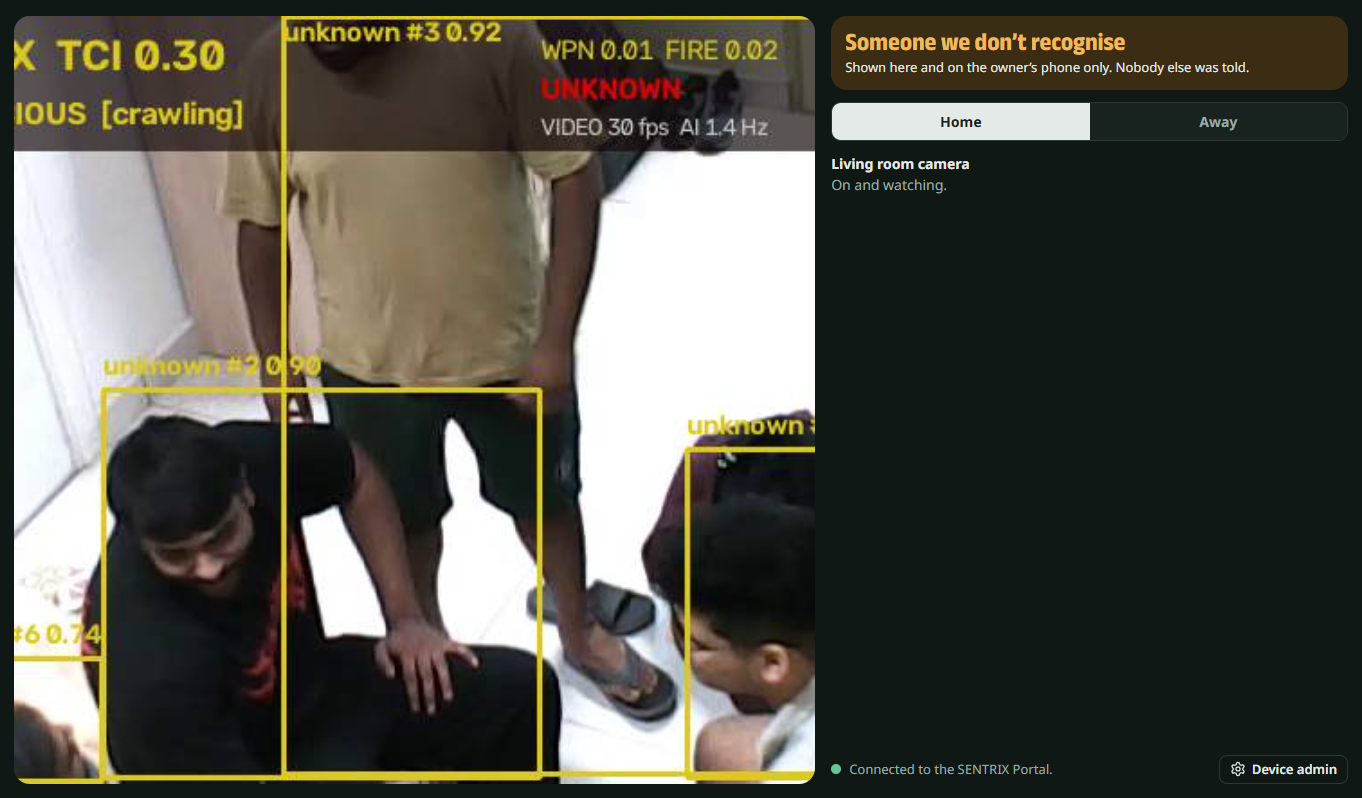
\includegraphics[width=0.49\textwidth]{figures/screens_c/dev_wall_idle.png}\hfill
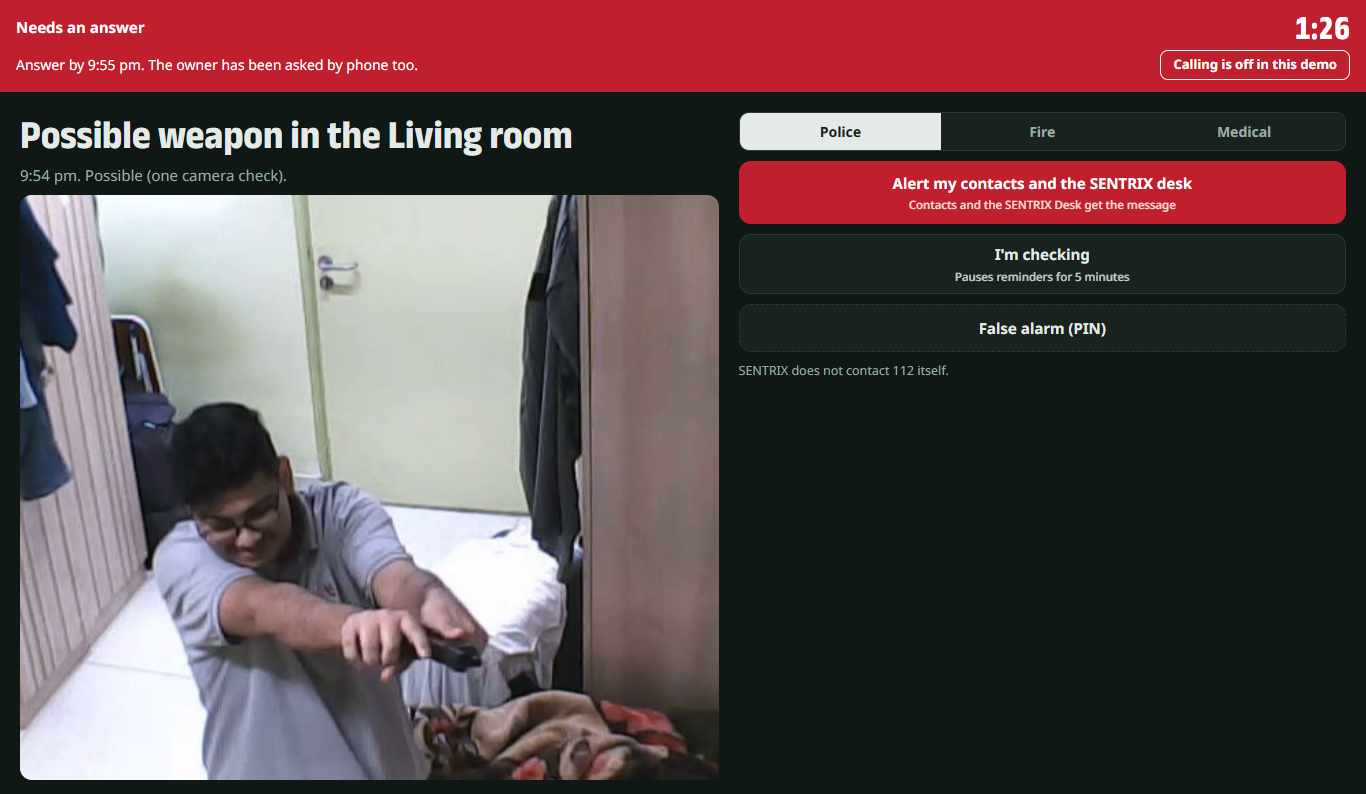
\includegraphics[width=0.49\textwidth]{figures/screens_c/dev_wall_alert.png}
\caption{Device screen: monitoring with tracked people labelled ``unknown'' (left) and the alert takeover after the handgun was confirmed, with countdown and answers (right)}
\label{fig:scr-wall}
\end{figure}

\begin{figure}[H]
\centering
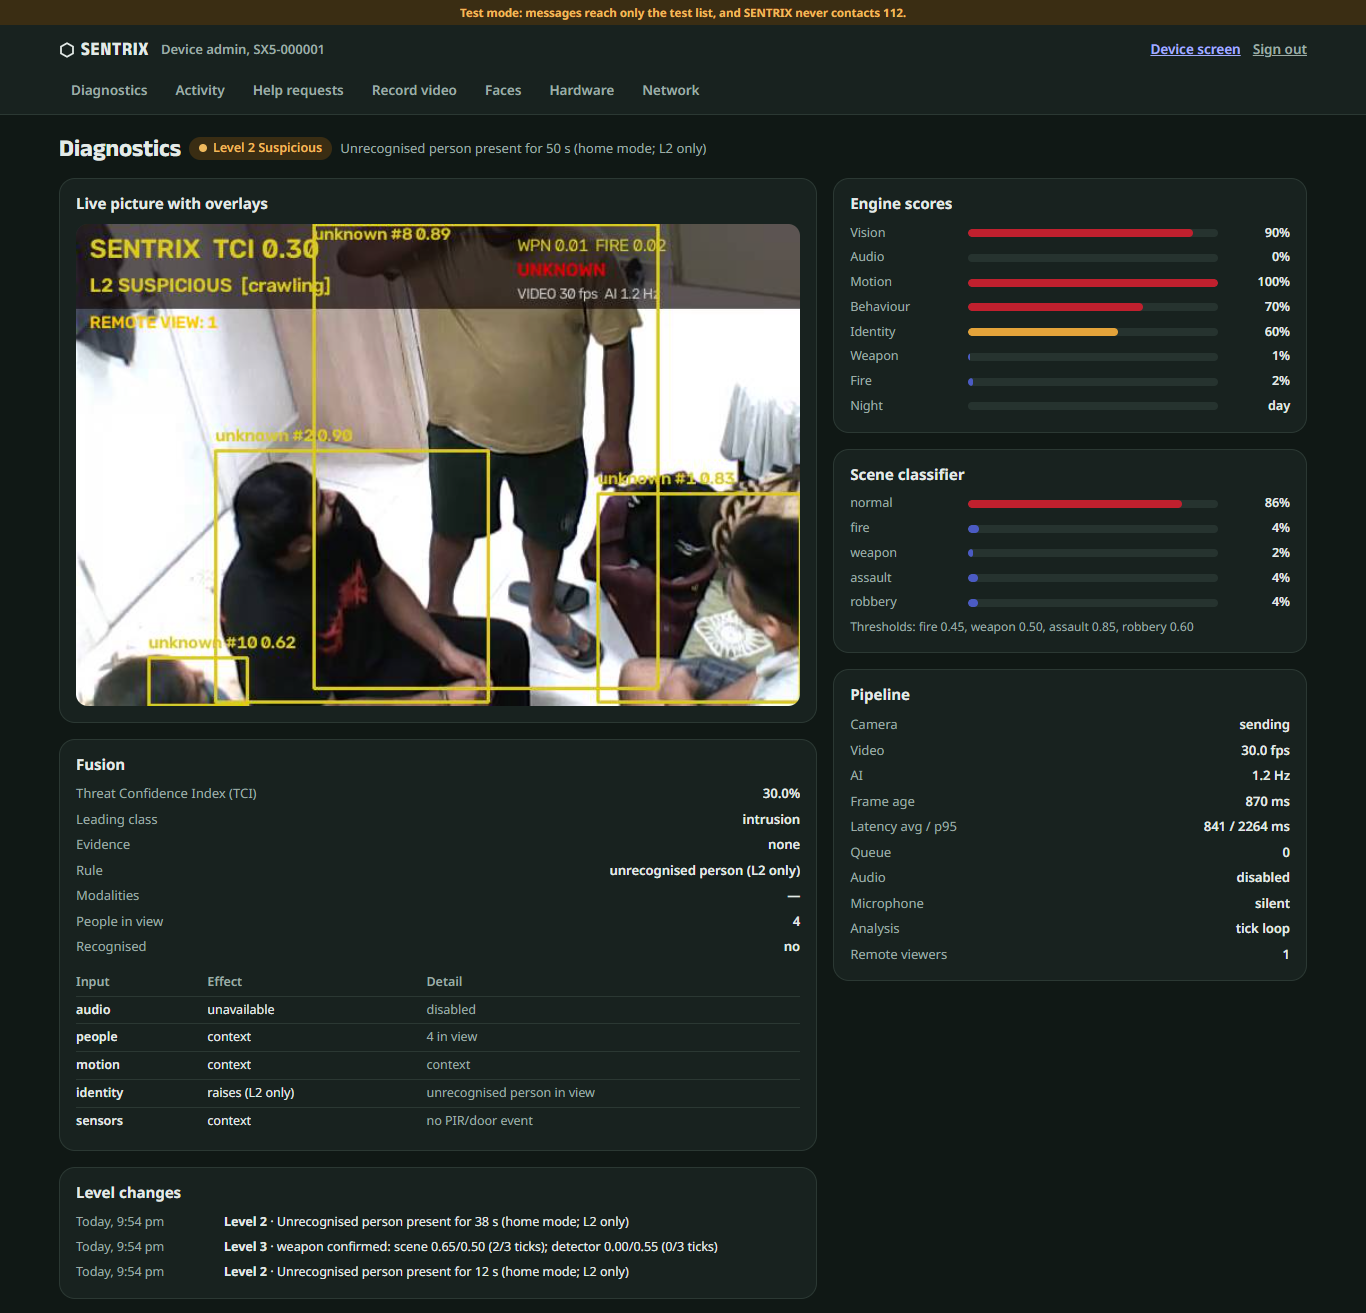
\includegraphics[width=0.92\textwidth]{figures/screens_c/dev_diagnostics.png}
\caption{Device administration, Diagnostics: live picture with overlays, model scores, scene probabilities with thresholds, the fusion result with the contribution of each input, and the level changes}
\label{fig:scr-diag}
\end{figure}

\begin{figure}[H]
\centering
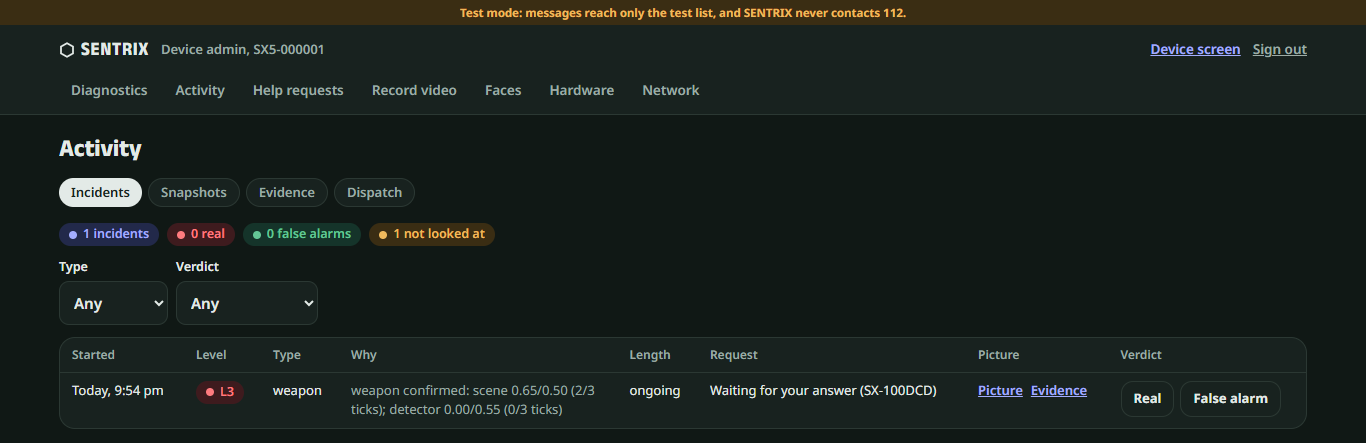
\includegraphics[width=0.49\textwidth]{figures/screens_c/dev_activity.png}\hfill
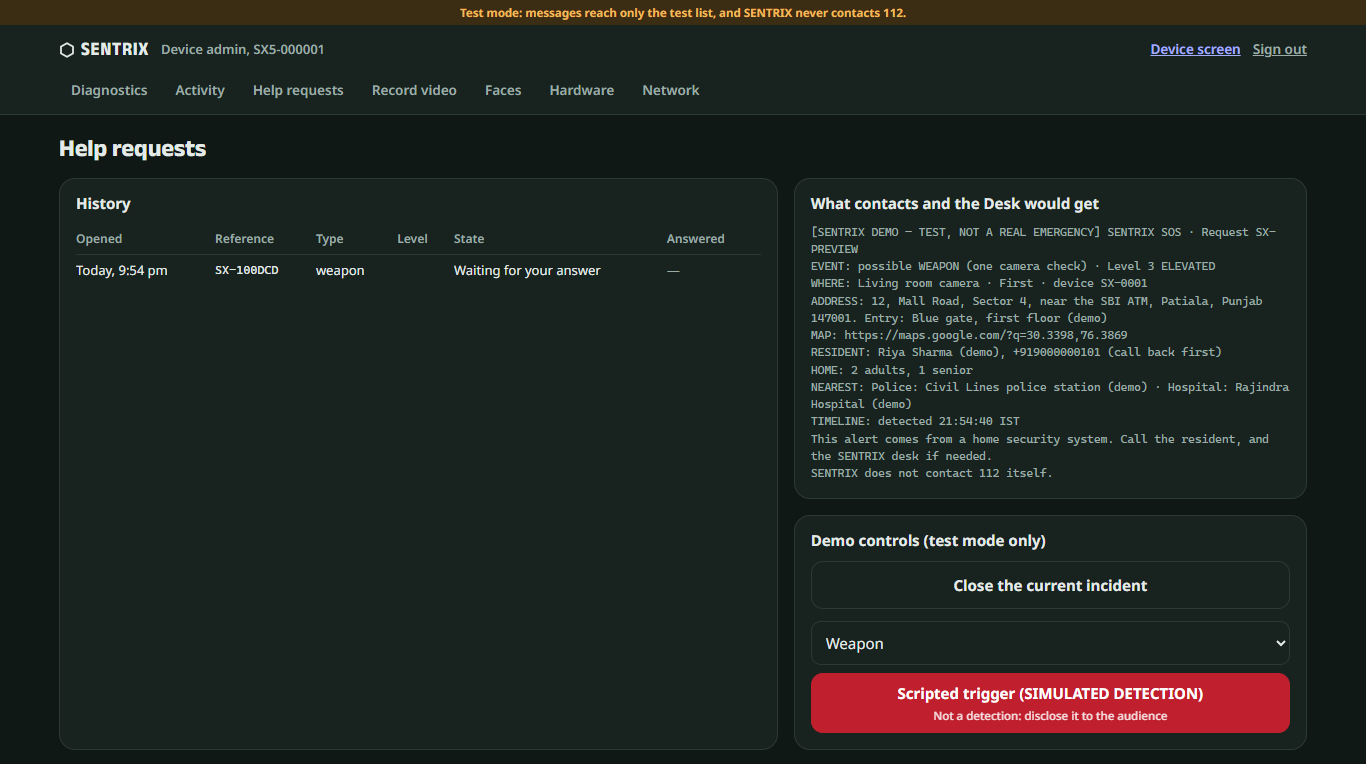
\includegraphics[width=0.49\textwidth]{figures/screens_c/dev_sos.png}
\caption{Device administration: Activity with the incident, its picture, evidence and verdict buttons (left); Help requests with the exact message contacts and the Desk would receive (right)}
\label{fig:scr-devadmin}
\end{figure}

\begin{figure}[H]
\centering
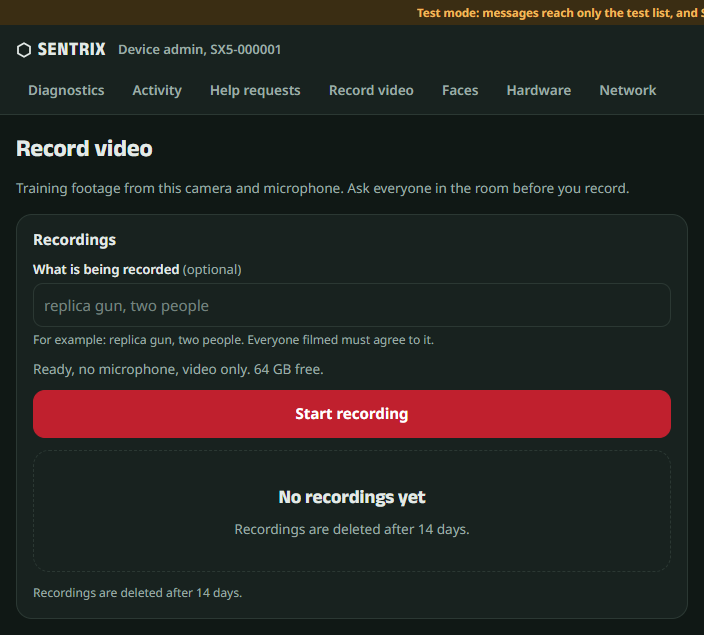
\includegraphics[width=0.36\textwidth]{figures/screens_c/dev_recordings.png}\hfill
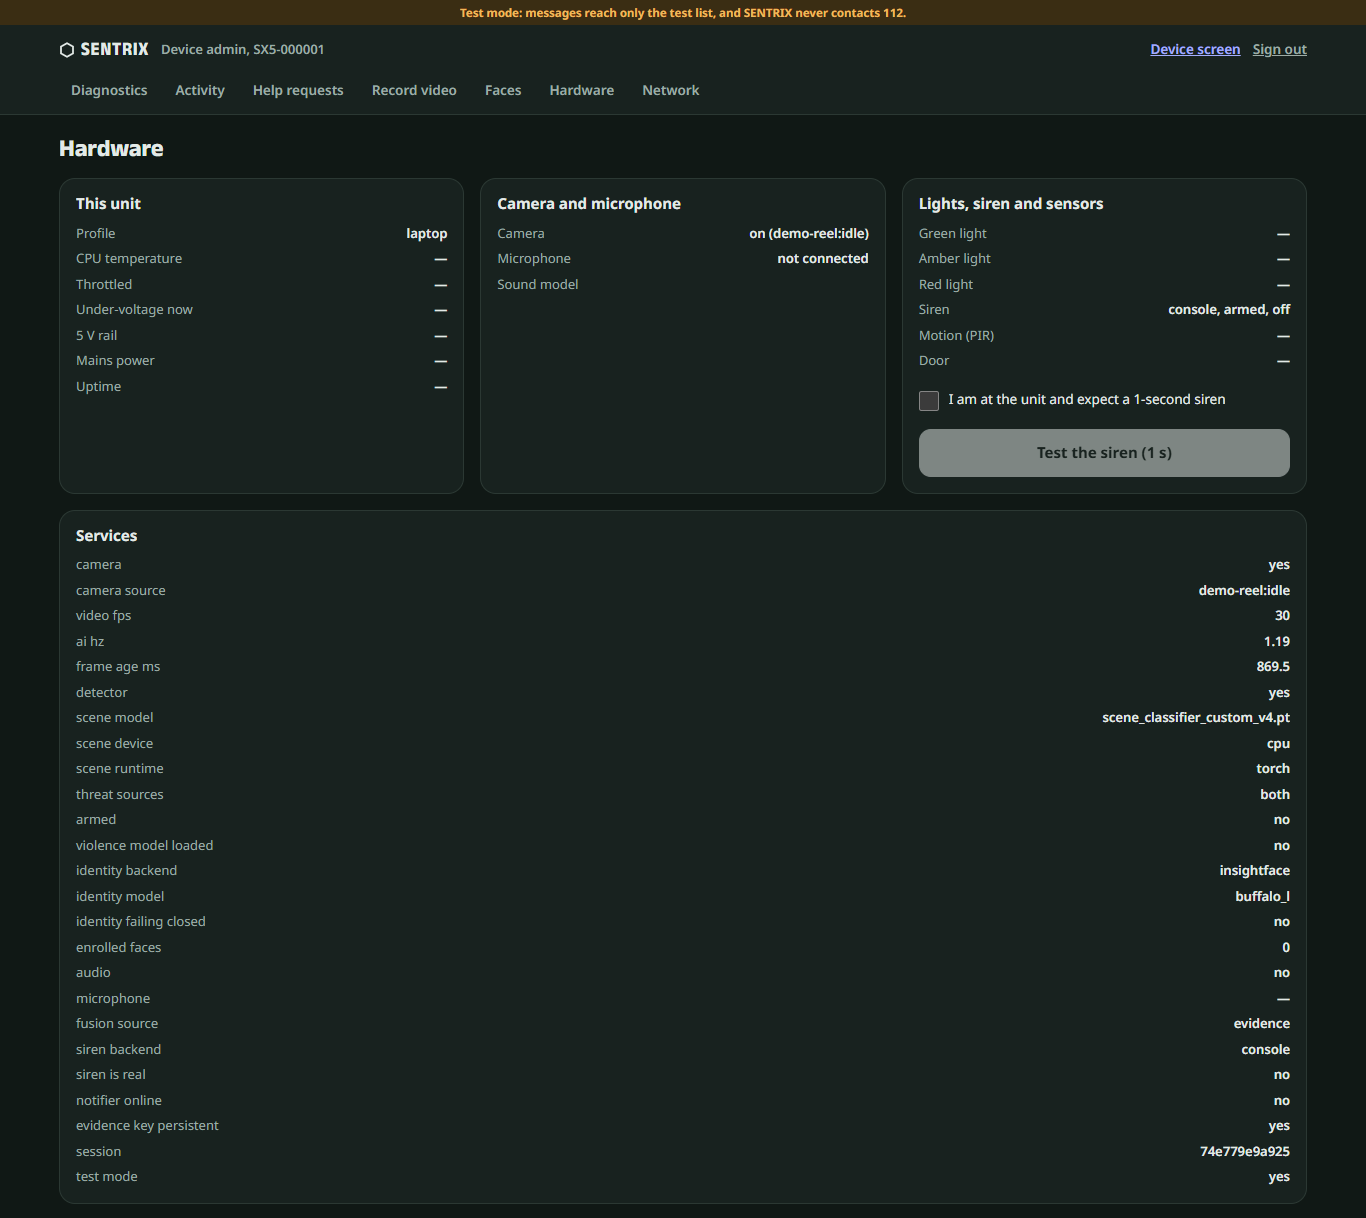
\includegraphics[width=0.62\textwidth]{figures/screens_c/dev_hardware.png}
\caption{Device administration: Record video for training data (left) and Hardware with services, LEDs, siren and sensors (right)}
\label{fig:scr-devhw}
\end{figure}

\begin{figure}[H]
\centering
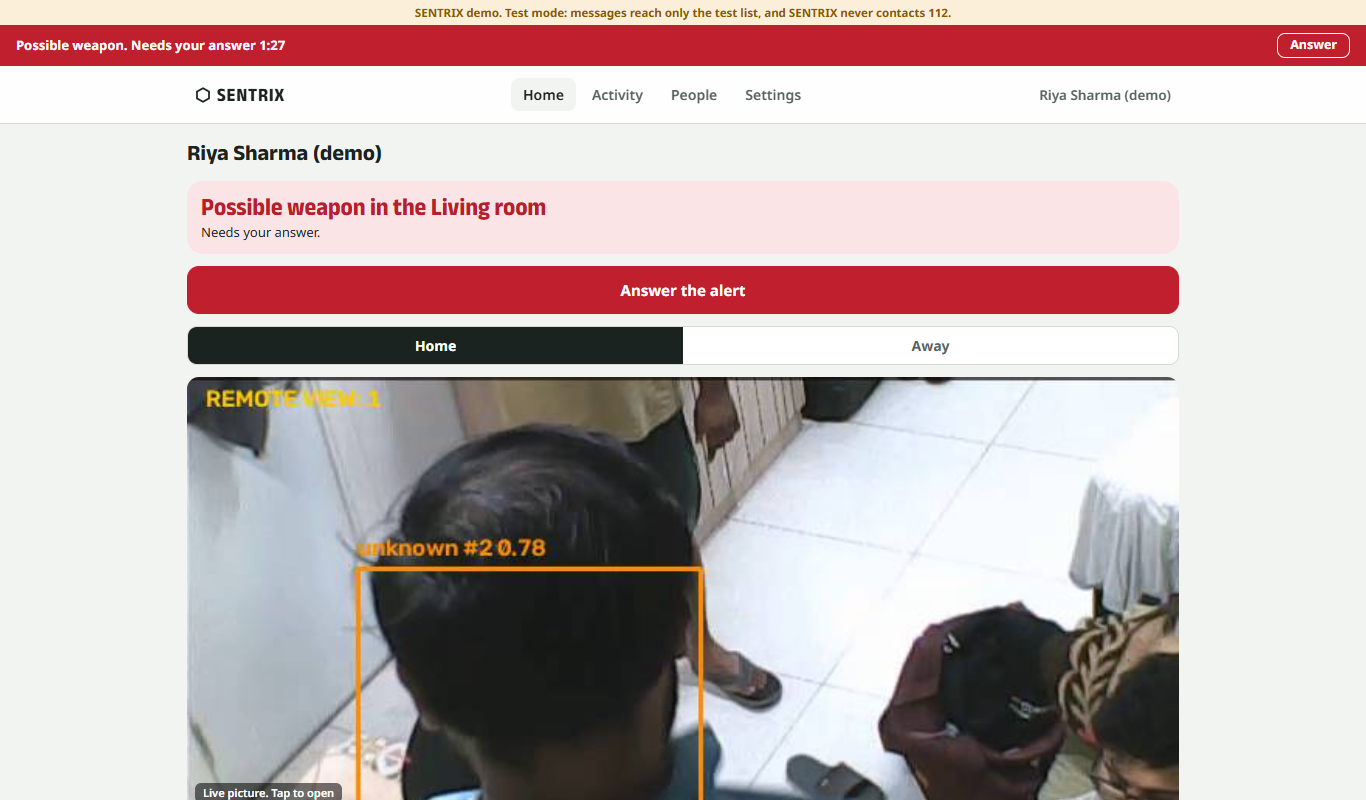
\includegraphics[width=0.60\textwidth]{figures/screens_c/portal_home_alert.png}\hfill
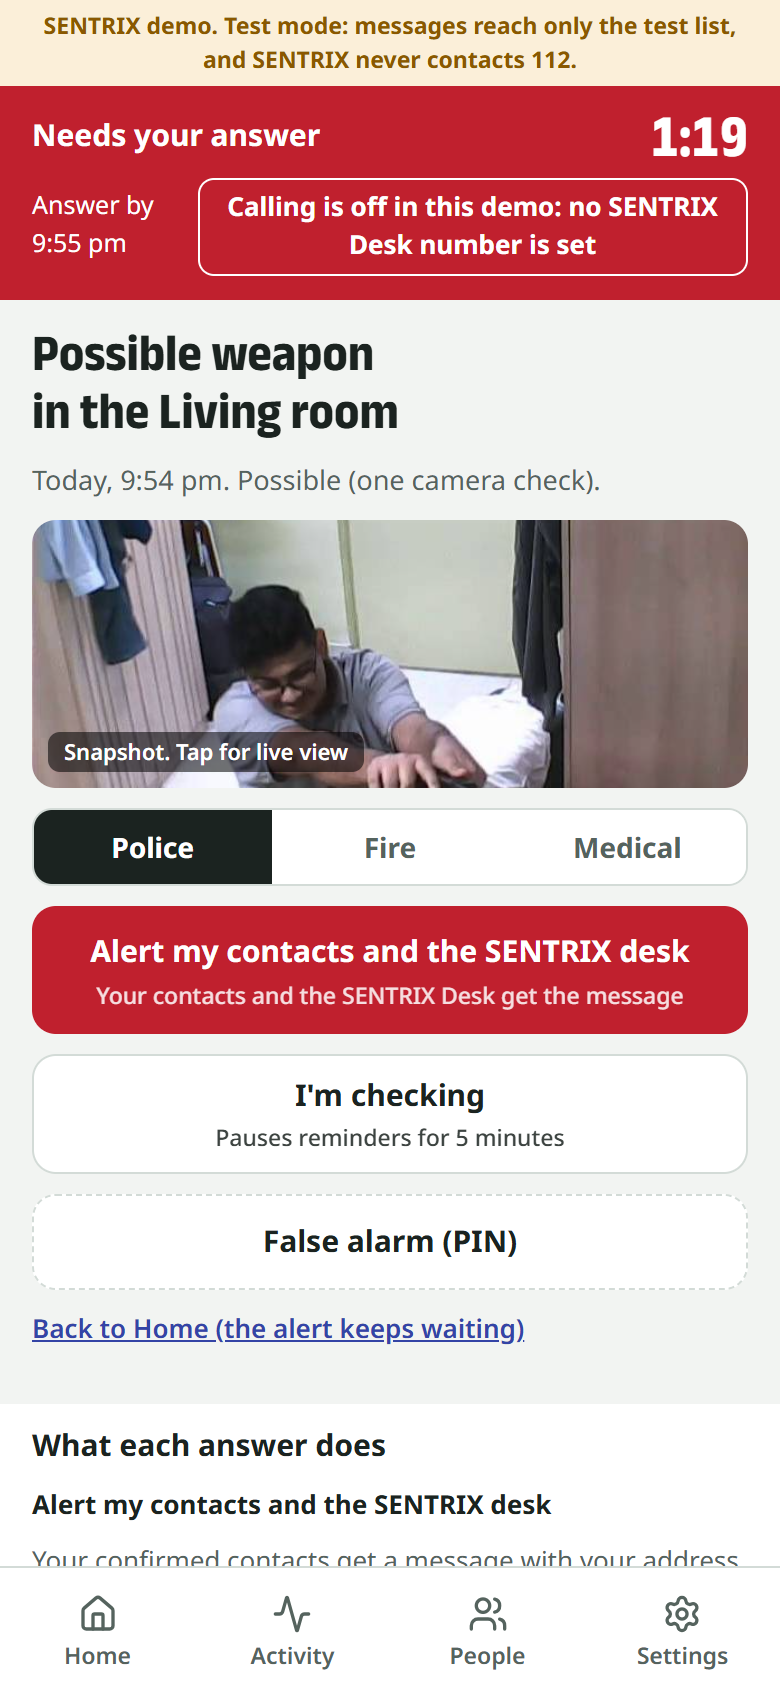
\includegraphics[width=0.36\textwidth]{figures/screens_c/portal_alert_phone.png}
\caption{Portal: the owner's home page with the red alert bar (left) and the alert screen on a phone, answers first (right)}
\label{fig:scr-alert}
\end{figure}

\begin{figure}[H]
\centering
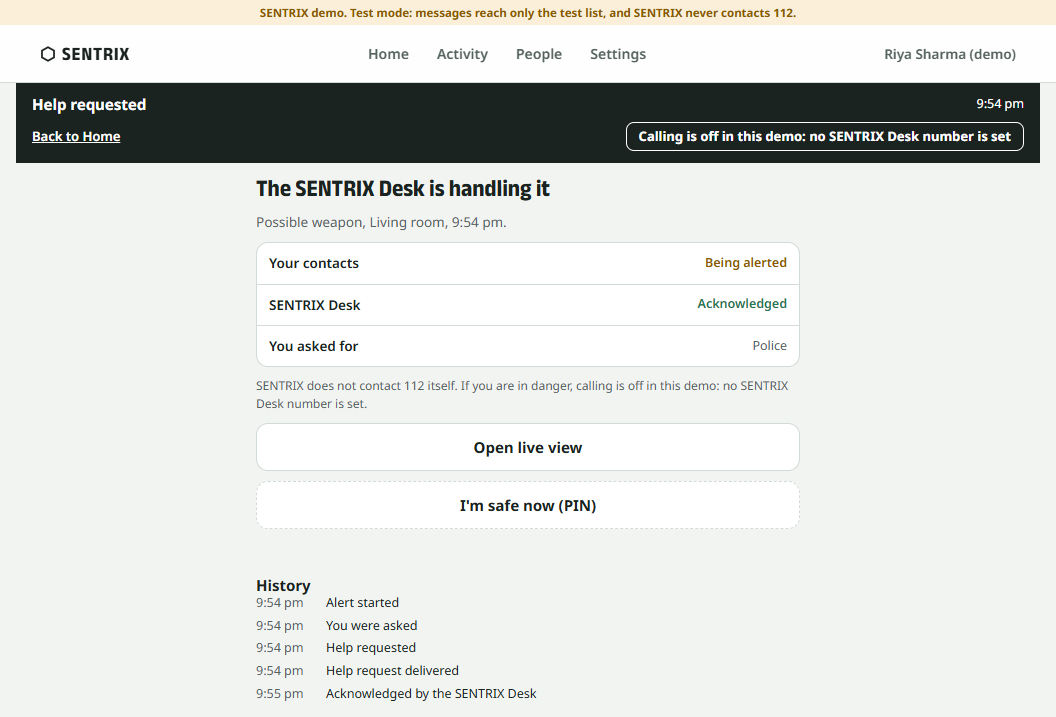
\includegraphics[width=0.49\textwidth]{figures/screens_c/portal_alert_ack.png}\hfill
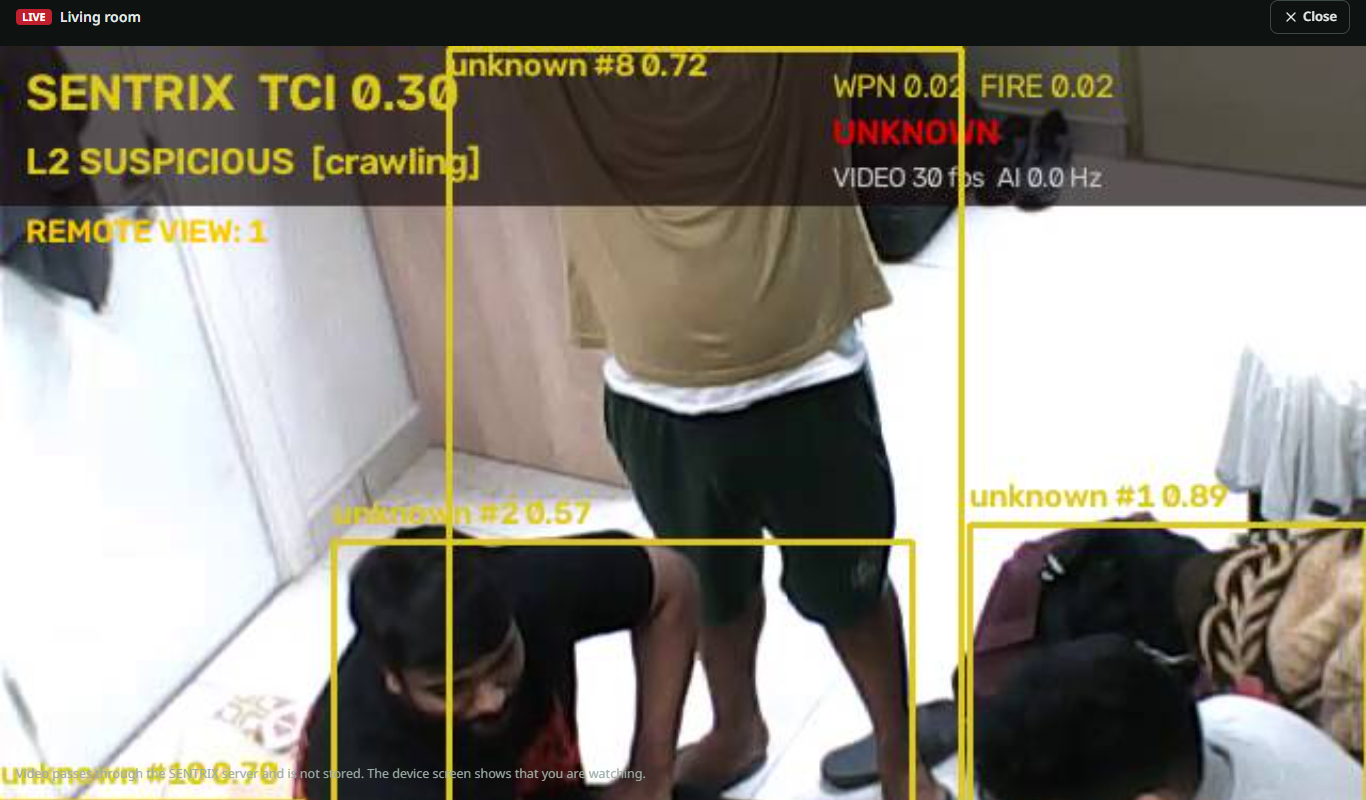
\includegraphics[width=0.49\textwidth]{figures/screens_c/portal_live.png}
\caption{Portal: after approval the owner sees ``The SENTRIX Desk is handling it'' with the timeline (left); live view of the device through the tunnel (right)}
\label{fig:scr-ack}
\end{figure}

\begin{figure}[H]
\centering
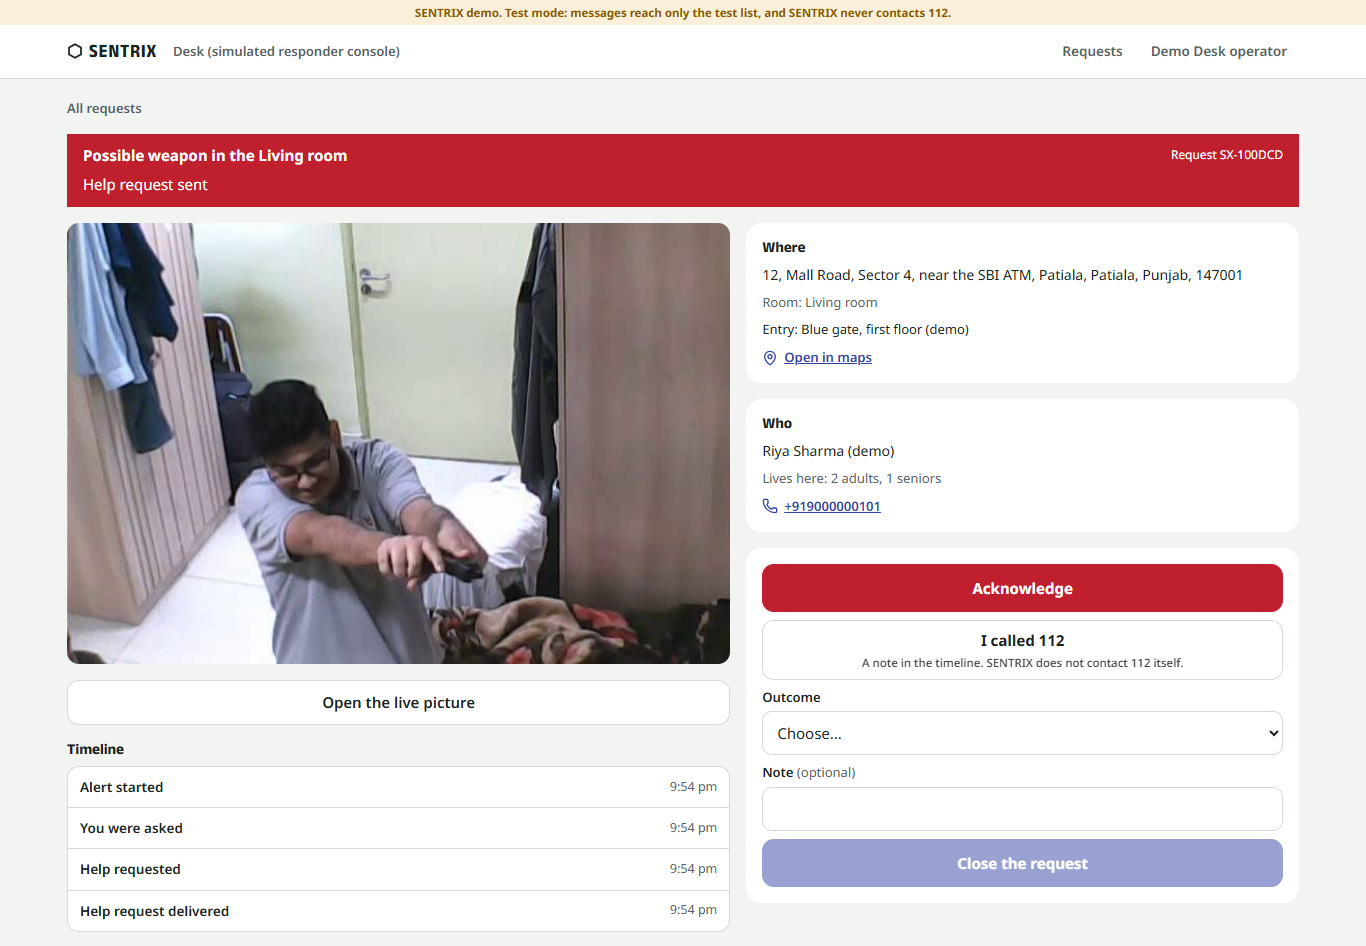
\includegraphics[width=0.66\textwidth]{figures/screens_c/desk_request.png}\hfill
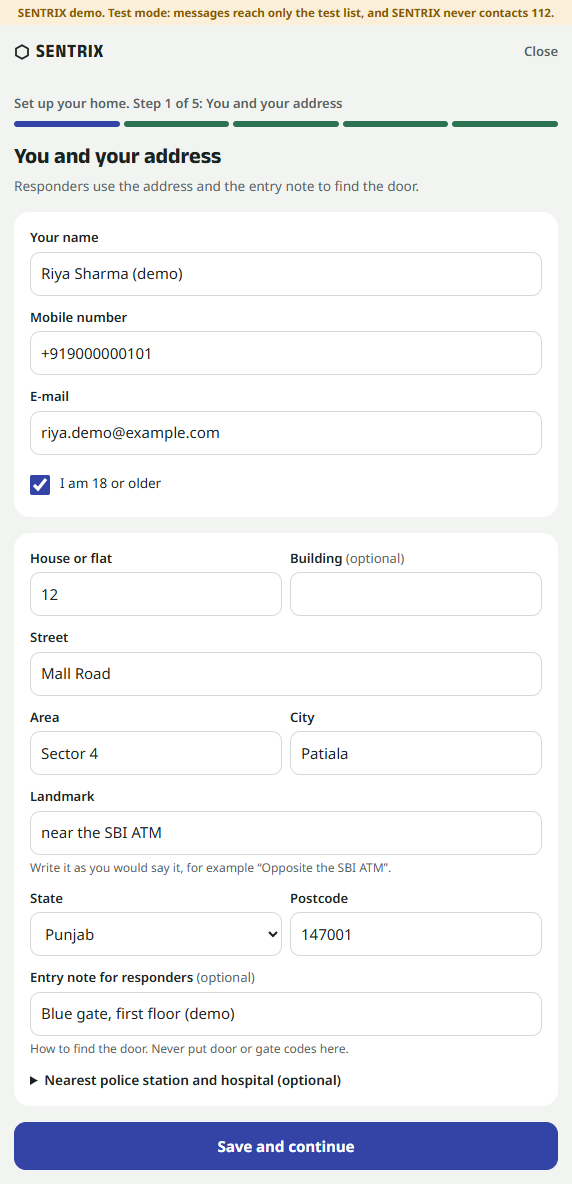
\includegraphics[width=0.32\textwidth]{figures/screens_c/portal_onboarding.png}
\caption{SENTRIX Desk request page with location, household, snapshot, acknowledge and close (left); onboarding wizard, step 1 (right)}
\label{fig:scr-desk}
\end{figure}

\begin{figure}[H]
\centering
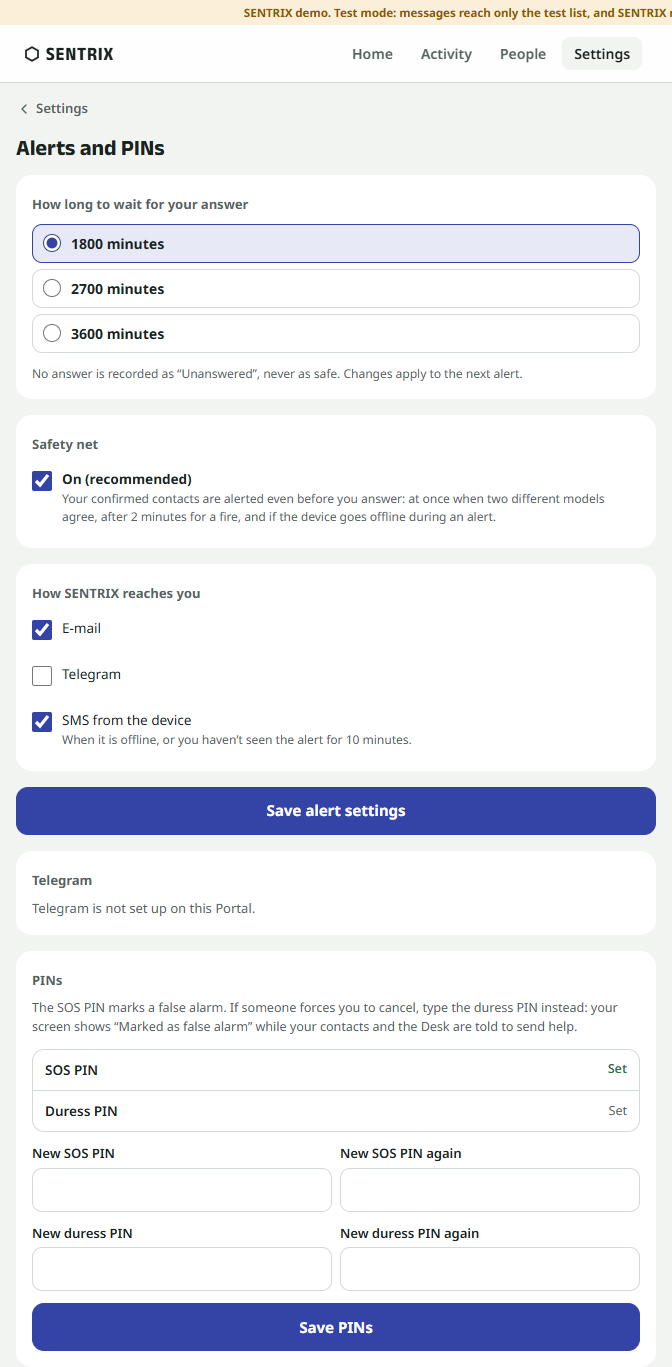
\includegraphics[width=0.32\textwidth]{figures/screens_c/portal_settings_alerts.png}\hfill
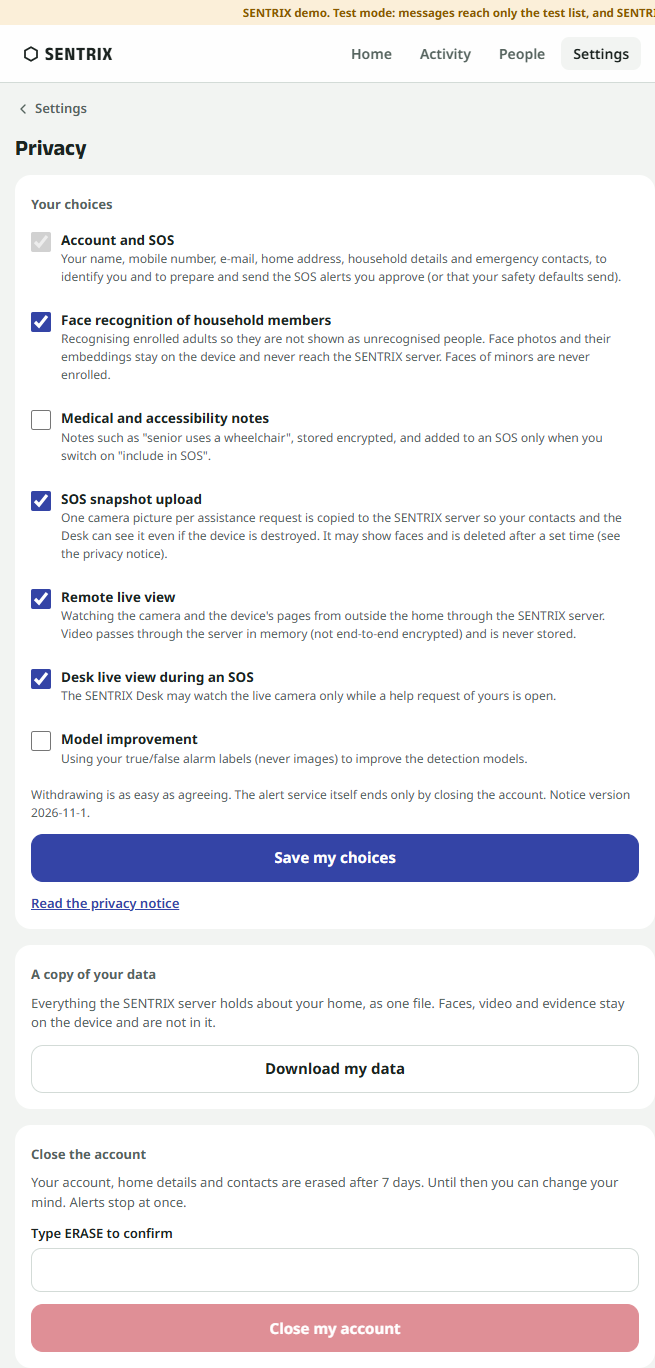
\includegraphics[width=0.32\textwidth]{figures/screens_c/portal_privacy.png}\hfill
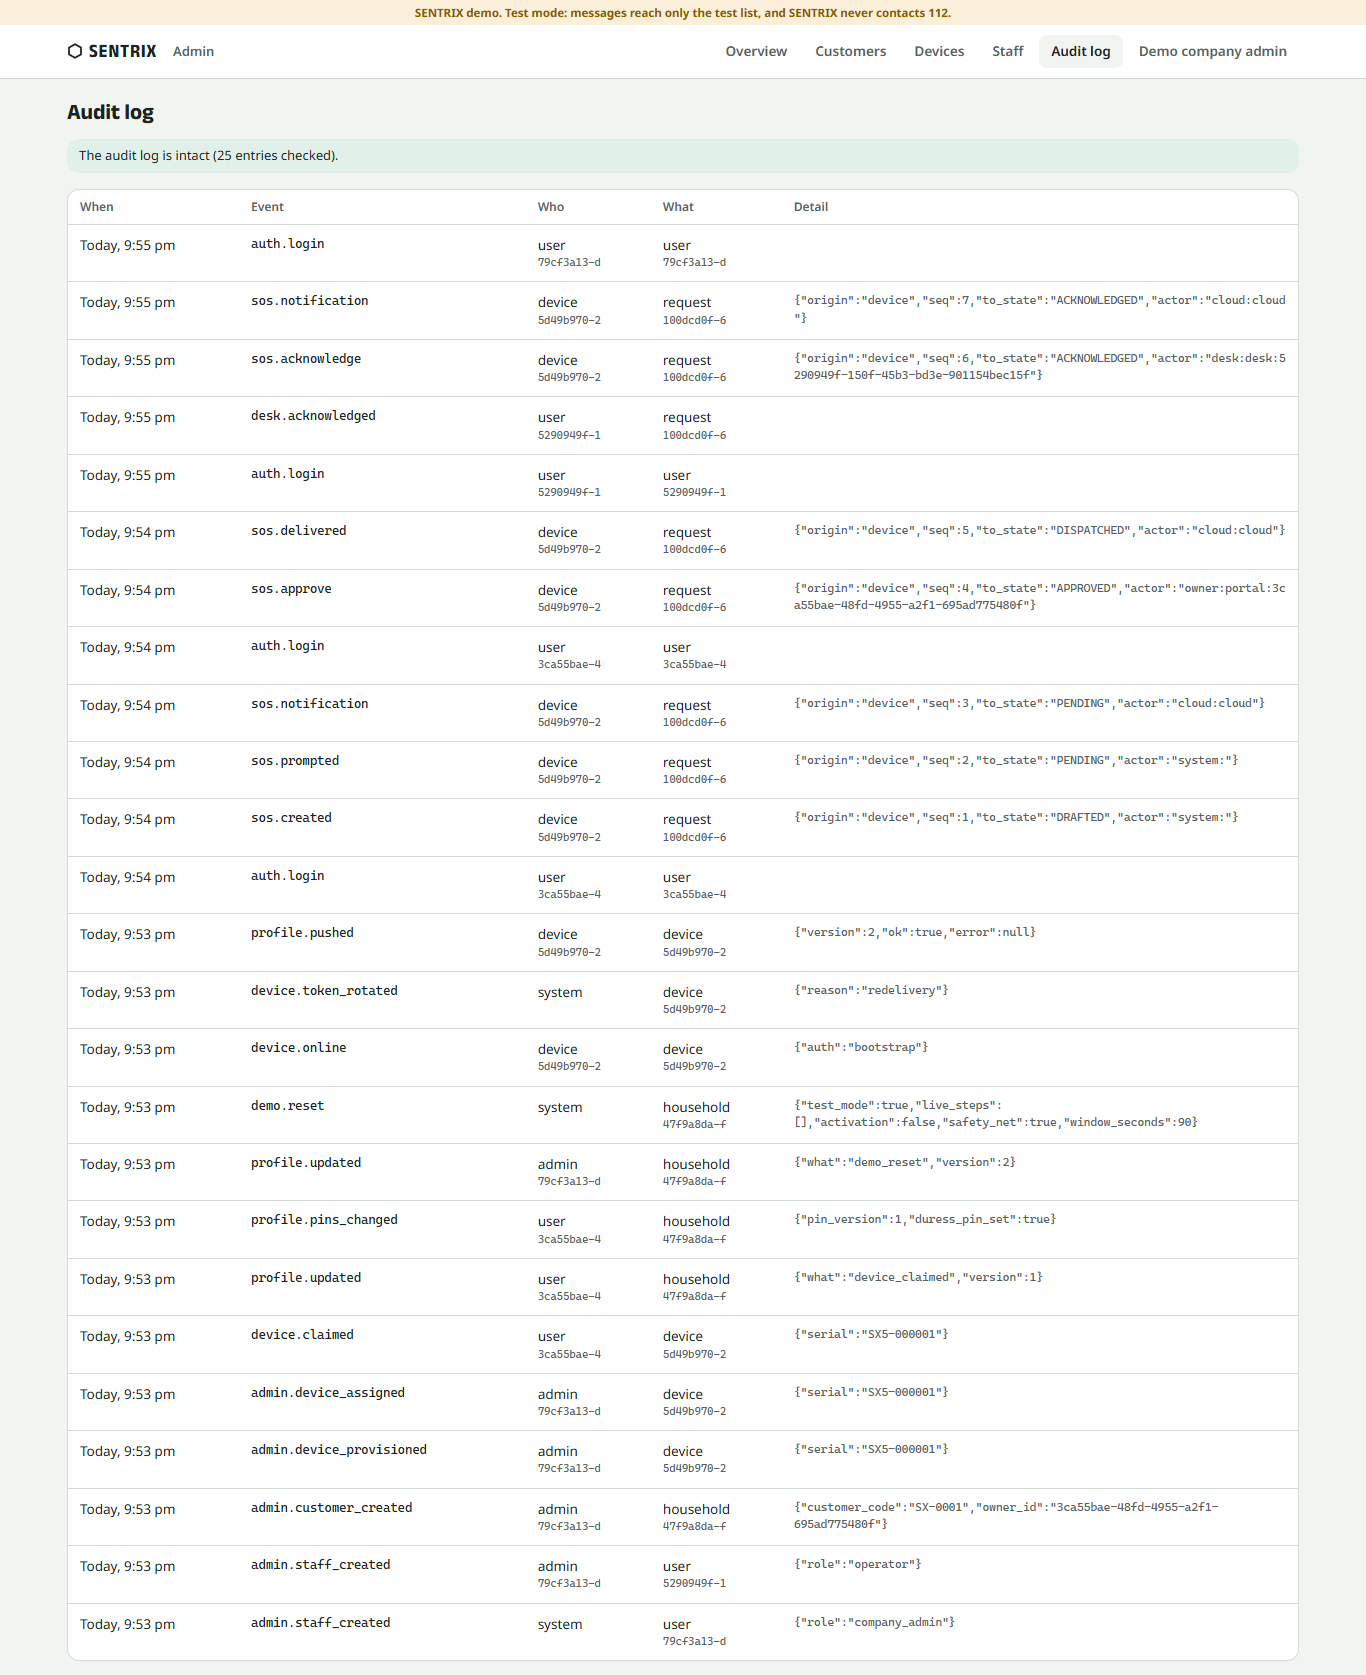
\includegraphics[width=0.32\textwidth]{figures/screens_c/admin_audit.png}
\caption{Portal: alert and PIN settings (left), privacy choices, export and erasure (centre), and the company audit log, whose hash chain is verified (right)}
\label{fig:scr-settings}
\end{figure}

%--------------------------------------------------------------
\section{Testing Process}
\label{sec:testing}

\subsection{Test Plan}
The test plan follows the structure of ISO/IEC/IEEE 29119-3 \cite{iso29119}.
\begin{itemize}
\item \textbf{Objective:} show that every requirement of Section~\ref{sec:srs} is met, that no test can ever send a real alert, and that detection performance is measured the way the product is used.
\item \textbf{Items under test:} the device package, the Portal, the two React applications, the deployment kits and the evaluation tools.
\item \textbf{Environment:} the laptop (Python 3.14, CPU), Microsoft Edge for browser tests; hardware behind fakes (gpiozero mock pins, fake Picamera2, fake \code{vcgencmd} and \code{/sys}, a fake AT-command serial port, fake Telegram/e-mail transports, a fake sound library).
\item \textbf{Isolation:} \code{tests/conftest.py} runs before any import: test mode on, every live switch off, provider keys blanked, the device's \code{var/} tree and the Portal database moved to a temporary directory, webcam and microphone blocked, and a socket guard that allows loopback only.
\item \textbf{Entry criteria:} code builds, the doctor tool passes. \textbf{Exit criteria:} the full suite passes; replay results equal or better than the previous milestone at Level~3 and above; no unexplained regression in benchmarks.
\item \textbf{Schedule:} the suite runs before every commit of a milestone (about 6.5 minutes); replays and benchmarks at every model or rule change.
\end{itemize}

\subsection{Features to be Tested}
Perception wrappers and model loading; evidence confirmation, corroboration, fight and banter rules; TCI and level policy; incidents, event log and evidence vault (including crash safety); per-track identity and body re-identification; audio alignment and the microphone chooser; the clip engine, fast lane and runtimes; the SOS machine, policy, PINs, sweeper and service; channels, outbox and the send guard; the link client, tunnel and path table; the Local Console API and its security (sessions, CSRF, CSP, rate limits); recordings; the Portal's accounts, onboarding, household, contacts, Desk, admin, privacy and retention; Pi hardware services; deployment kits; and the end-to-end product flow.

\subsection{Test Strategy}
Testing is layered (\figref{fig:tests}):
\begin{enumerate}
\item \textbf{Unit tests} for pure logic (the SOS machine, evidence rules, policy, resampler, recorder frame grid).
\item \textbf{Integration tests} for each service with its real neighbours and fake transports (channels with fake Telegram and modem; the link client against the Portal hub over an in-memory pipe).
\item \textbf{In-process product tests:} \code{tests/test\_e2e\_product.py} runs the Portal, the device console with a fake pipeline, the real SOS engine on an injected clock and the real link client in one event loop through 13 scenarios.
\item \textbf{Browser end-to-end tests:} Playwright drives Microsoft Edge against the real Portal and device processes in a fresh test-mode demo world, at desktop and phone sizes.
\item \textbf{Evaluation as regression:} replay of the ten labelled videos and of the recorded live session after every change to rules or models.
\item \textbf{Live smoke runs and reviews:} the Portal and the device as two real processes linked over a real WebSocket, and adversarial reviews in which each finding needs a concrete failing case before it is fixed.
\end{enumerate}

\begin{figure}[htbp]
\centering
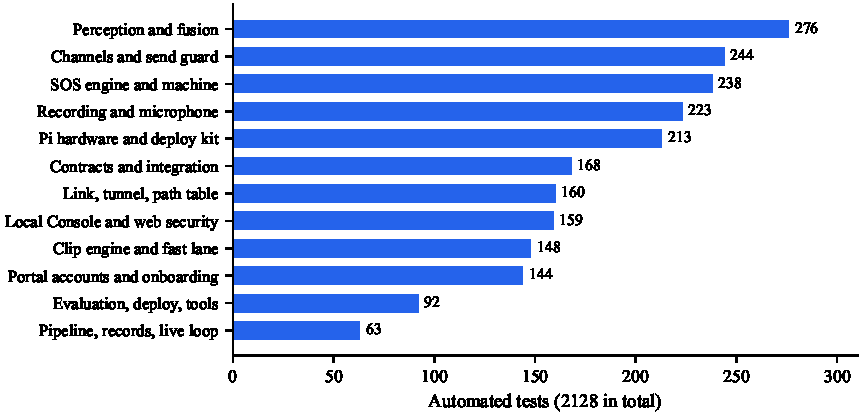
\includegraphics[width=0.85\textwidth]{figures/fig_tests.pdf}
\caption{Automated tests per area (2128 collected on the device and Portal branch)}
\label{fig:tests}
\end{figure}

\subsection{Test Techniques}
\begin{itemize}
\item \textbf{Equivalence partitioning and boundary values:} scores exactly at a threshold, 1 of 3 versus 2 of 3 confirmations, gaps just under and over 3\,s, dwell times of 0.59 and 0.61\,s, recordings at the 2\,GB floor.
\item \textbf{State-transition testing:} every allowed and forbidden transition of the SOS table, duress parity (the owner's screens after a duress PIN must equal a normal false alarm), reconnect merges.
\item \textbf{Time travel:} the SOS engine and the Portal workers run on an injected clock, so 30-minute windows, reminders and safety defaults are tested in milliseconds.
\item \textbf{Fault injection:} 100 forced link disconnects (no event lost), \code{taskkill /F} during an open incident (no event row lost), a real \code{os.\_exit} crash during a recording (the partial files are recovered), a modem that browns out, Telegram returning errors.
\item \textbf{Security tests:} CSRF without a token, cross-household access, XSS in names, the tunnel's path table per role, secrets never in a response, rate limits.
\item \textbf{Replay regression:} the recorded live session re-decided under each new rule set.
\end{itemize}

\subsection{Test Cases}
\tabref{tab:testcases} lists representative test cases; each is an automated test in the repository.

\begin{longtable}{|C{0.95cm}|L{2.9cm}|L{4.3cm}|L{3.4cm}|C{0.95cm}|}
\caption{Representative test cases}\label{tab:testcases}\\
\hline\rowhead
\thead{ID} & \thead{Feature (test file)} & \thead{Input / steps} & \thead{Expected result} & \thead{Result}\\ \hline
\endfirsthead
\hline\rowhead
\thead{ID} & \thead{Feature (test file)} & \thead{Input / steps} & \thead{Expected result} & \thead{Result}\\ \hline
\endhead
\multicolumn{5}{r}{\footnotesize\itshape continued on next page}\\
\endfoot
\endlastfoot
\tablefont TC-01 & \tablefont Confirmation (test\_evidence) & \tablefont One scene vote over threshold, then two below & \tablefont Not confirmed; TCI below Level~2 & \tablefont Pass\\ \hline
\tablefont TC-02 & \tablefont Confirmation (test\_evidence) & \tablefont A cached value carried on later ticks & \tablefont Does not count again; never confirms itself & \tablefont Pass\\ \hline
\tablefont TC-03 & \tablefont Person gate & \tablefont Weapon votes with no person for 2.5\,s & \tablefont Weapon gated, no alarm & \tablefont Pass\\ \hline
\tablefont TC-04 & \tablefont Corroboration (test\_multimodal) & \tablefont Pistol box + gunshot sound aligned & \tablefont Level~4 & \tablefont Pass\\ \hline
\tablefont TC-05 & \tablefont Audio alone & \tablefont Scream with no visual source & \tablefont At most Level~2, never a weapon & \tablefont Pass\\ \hline
\tablefont TC-06 & \tablefont Banter & \tablefont Video fight + aligned laughter & \tablefont Held at Level~2, labelled banter & \tablefont Pass\\ \hline
\tablefont TC-07 & \tablefont Stale audio & \tablefont Audio window 3\,s before the frame & \tablefont Audio ``unavailable'', no vote & \tablefont Pass\\ \hline
\tablefont TC-08 & \tablefont Unknown person & \tablefont Stranger present 10\,s at home & \tablefont Level~2 only, no snapshot, no SOS & \tablefont Pass\\ \hline
\tablefont TC-09 & \tablefont Level policy (test\_fusion) & \tablefont TCI ramp rising across several bands & \tablefont Each level commits as earned; L4/L5 after 0.6\,s and 2 observations & \tablefont Pass\\ \hline
\tablefont TC-10 & \tablefont Records (test\_records) & \tablefont Incident row left open by a crash & \tablefont Every event row on disk before close; open row closed at the next start & \tablefont Pass\\ \hline
\tablefont TC-11 & \tablefont Evidence (test\_clip\_engine) & \tablefont Two clip bundles sealed & \tablefont Manifest hash chain verifies with 2 entries & \tablefont Pass\\ \hline
\tablefont TC-12 & \tablefont Identity (test\_identity) & \tablefont Resident and stranger in view (tailgating) & \tablefont Stranger stays unknown & \tablefont Pass\\ \hline
\tablefont TC-13 & \tablefont Re-id (test\_reid) & \tablefont Armed mode, body matches resident & \tablefont Not authorised (face only) & \tablefont Pass\\ \hline
\tablefont TC-14 & \tablefont SOS machine (test\_sos\_machine) & \tablefont Confirmed weapon L3 & \tablefont One request DRAFTED $\to$ PENDING; later incidents attach & \tablefont Pass\\ \hline
\tablefont TC-15 & \tablefont SOS expiry & \tablefont No answer for the whole window & \tablefont EXPIRED, labelled ``Unanswered'', never ``safe'' & \tablefont Pass\\ \hline
\tablefont TC-16 & \tablefont Duress (test\_sos\_engine) & \tablefont Duress PIN entered & \tablefont Screen shows false alarm; contacts and Desk alerted & \tablefont Pass\\ \hline
\tablefont TC-17 & \tablefont PIN lockout (test\_sos\_pins) & \tablefont Five wrong PINs & \tablefont Answers locked for 10 minutes & \tablefont Pass\\ \hline
\tablefont TC-18 & \tablefont Safety default & \tablefont Fire request unanswered for 2 min & \tablefont Confirmed contacts alerted & \tablefont Pass\\ \hline
\tablefont TC-19 & \tablefont Send guard (test\_ch\_router) & \tablefont Message to 112 with live switches on & \tablefont Always refused & \tablefont Pass\\ \hline
\tablefont TC-20 & \tablefont Test mode & \tablefont Recipient not on the allowlist & \tablefont SUPPRESSED, nothing sent & \tablefont Pass\\ \hline
\tablefont TC-21 & \tablefont Link (test\_integration\_m10) & \tablefont 100 forced disconnects & \tablefont 0 events lost after reconnect & \tablefont Pass\\ \hline
\tablefont TC-22 & \tablefont Path table (test\_link\_policy) & \tablefont Tunnelled request for a LAN-only page or an unknown write & \tablefont Refused & \tablefont Pass\\ \hline
\tablefont TC-23 & \tablefont Isolation (test\_acct\_isolation) & \tablefont Owner A requests household B's data & \tablefont 403/404, nothing leaked & \tablefont Pass\\ \hline
\tablefont TC-24 & \tablefont Siren (test\_hw\_siren) & \tablefont Activation of 120\,s & \tablefont Released after at most 90\,s & \tablefont Pass\\ \hline
\tablefont TC-25 & \tablefont Recorder (test\_recorder) & \tablefont Crash by \code{os.\_exit} while recording & \tablefont Partial files recovered at next start & \tablefont Pass\\ \hline
\tablefont TC-26 & \tablefont Product flow (test\_e2e\_product) & \tablefont Provision $\to$ activate $\to$ onboard $\to$ claim $\to$ L3 $\to$ approve $\to$ Desk & \tablefont Request CLOSED, verdict TRUE & \tablefont Pass\\ \hline
\tablefont TC-27 & \tablefont Browser: alert journey (sos.spec) & \tablefont Scripted weapon; owner answers; Desk acknowledges and closes & \tablefont Every screen updates; no \code{tel:112} link in test mode & \tablefont Pass\\ \hline
\tablefont TC-28 & \tablefont Browser: false alarm on a phone & \tablefont Wrong PIN, then the right PIN & \tablefont Wrong PIN refused; marked as false alarm & \tablefont Pass\\ \hline
\tablefont TC-29 & \tablefont Browser: add a contact (owner.spec) & \tablefont Owner adds an emergency contact & \tablefont Confirmation step with a one-time link shown & \tablefont \textbf{Fail}\\ \hline
\end{longtable}

\subsection{Test Results}
\label{sec:test-results}
\begin{itemize}
\item \textbf{Device and Portal suite} (branch \code{sentrix/portal}, commit \code{5127b3c}, with body re-identification, the v5 detector heads and room calibration): \textbf{2154 passed} in 386.6\,s on the laptop. The device guard blocked 4 webcam/microphone attempts and the socket guard 2 network attempts---all made deliberately by the tests that check those guards.
\item \textbf{Frontend branch} (\code{sentrix/frontend-v2}, commit \code{c1241c1}, the React applications): Python suite \textbf{2243 passed, 1 skipped} in 385.4\,s; Vitest unit tests \textbf{15 of 15} passed; Playwright browser tests \textbf{22 of 23} passed at desktop and phone sizes. The failing case (TC-29) is the owner adding an emergency contact: the page did not show the ``ask the contact to confirm'' step within 15\,s. It is a known defect to be fixed before the final demonstration; adding contacts through onboarding is covered by passing tests.
\item \textbf{Live smoke run} (Portal and device as two real processes linked over a real WebSocket, demo reel): every Local Console page and 14 GET APIs gave the same status directly and through the tunnel; ``scene gun'' produced a PENDING weapon request 8.0--9.8\,s after the clip started and ``scene fire'' 11.6--11.9\,s; approval reached the device as DISPATCHED in 0.01--0.28\,s; MJPEG ran at 29.9\,fps directly and 13.6\,fps through the tunnel (cap 15). Five defects found in the run were fixed with regression tests.
\item \textbf{Live on the Raspberry~Pi~5 with the Render Portal and Telegram:} detections in the demo room opened assistance requests that were prompted on the Pi's screen and the owner's phone; requests were declined with the PIN, expired unanswered, and in one case approved, dispatched and resolved on the Desk. These were false alarms from the scene classifier in the new room, and they are the data from which the room thresholds were set (Section~\ref{sec:results}).
\item \textbf{Bug sweep and audits:} a five-way code audit and a twelve-item bug sweep (October 2026) and a wiring and copy audit (November 2026) each fixed every confirmed finding with a regression test.
\end{itemize}

%--------------------------------------------------------------
\section{Results and Discussions}
\label{sec:results}

\subsection{Choosing the models}
\figref{fig:configs} compares the three model configurations on the held-out validation videos and on the replay of all ten videos. The models trained on the team's own footage (v4: DINOv2 scene classifier and YOLO11n heads) nearly doubled validation macro-F1 over the fine-tuned v3 models (0.768 vs 0.401) and cut false alarms per normal minute by a factor of nine (0.79 vs 7.12); the evidence rules of M1 then removed the remaining false alarms (0.00) while keeping the same 13 of 18 episodes. The one clear loss of v4 is the test corridor's swung stick, which it never detects (0 of 3 episodes): 39 frames of a stick \emph{carried} in one training video did not teach a stick \emph{swung} in another. Stick is therefore experimental in the product.

\begin{figure}[htbp]
\centering
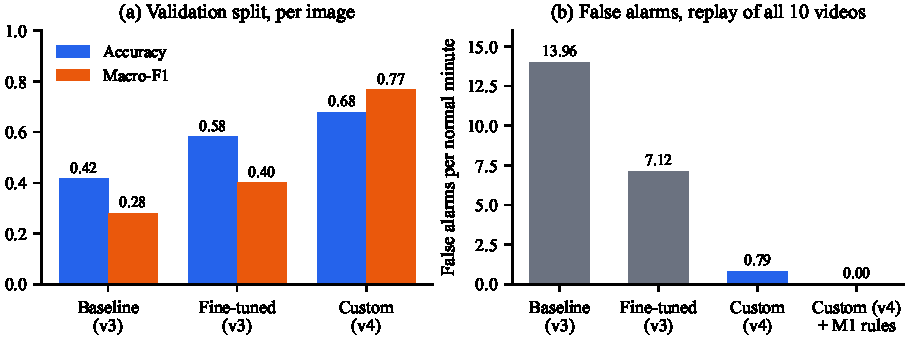
\includegraphics[width=\textwidth]{figures/fig_configs.pdf}
\caption{Model configurations on the custom dataset: (a) validation accuracy and macro-F1 per image; (b) false alarms per minute of normal footage in the replay of all ten videos}
\label{fig:configs}
\end{figure}

\begin{table}[htbp]
\caption{Held-out results of the three configurations (validation: gun, vid04; test: wa02)}
\label{tab:configs}
\centering\tablefont
\begin{tabularx}{\textwidth}{|Y|C{2.6cm}|C{2.6cm}|C{2.6cm}|}
\hline\rowhead
\thead{Measure} & \thead{Baseline (v3)} & \thead{Fine-tuned (v3)} & \thead{Custom (v4)}\\ \hline
Validation per image: accuracy / macro-F1 & 0.417 / 0.281 & 0.583 / 0.401 & \textbf{0.679 / 0.768}\\ \hline
Validation replay: episodes / false alarms & 1 of 2 / 0 & 1 of 2 / 4 & \textbf{2 of 2 / 0}\\ \hline
Test per image: accuracy / macro-F1 & 0.043 / 0.114 & 0.677 / \textbf{0.460} & \textbf{0.720} / 0.419\\ \hline
Test replay: stick episodes & 3 of 3 (alarms on everything) & \textbf{3 of 3} & 0 of 3\\ \hline
False alarms per normal minute, all 10 videos & 13.96 & 7.12 & \textbf{0.79}\\ \hline
Leave-one-video-out macro-F1 of the scene model & -- & 0.210 & \textbf{0.440}\\ \hline
\end{tabularx}
\end{table}

\subsection{Effect of the evidence rules}
\figref{fig:livesession} re-decides the first live session under the rules of each stage. As logged, the old pipeline committed 30 onsets at Level~2 and above, 9 at Level~3 and 6 at Level~4 in 18.3 minutes. Under the M1 rules the same log gives 0, 0 and 0. Under the final rules (D15) it gives 5 Level~2 onsets---the by-design ``someone we don't recognise'' notices for unenrolled team members---and still 0 at Level~3 and above. The cost was latency: on the held-out handgun video the first Level~3 came 6.3\,s after the episode began instead of 2.4\,s, because the scene probability stays under the raised 0.50 floor for the first seconds.

\begin{figure}[htbp]
\centering
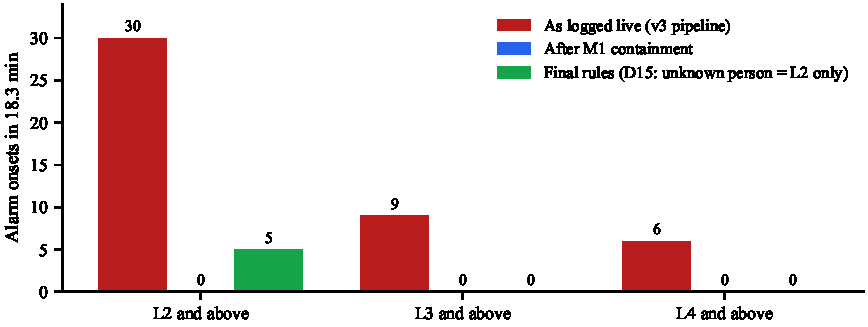
\includegraphics[width=0.92\textwidth]{figures/fig_live_session.pdf}
\caption{The first live session (18.3 minutes, laptop webcam) re-decided under each rule set}
\label{fig:livesession}
\end{figure}

\subsection{Detection per committed level}
\figref{fig:levels} and \tabref{tab:levels-res} show what reaches each level when the ten videos are replayed through the final pipeline with their own soundtracks. Three quarters of the handgun episodes and all flame episodes reach Level~3 (assistance request); half the handgun episodes and two of three flames are corroborated to Level~4; two handgun episodes and two flames reach Level~5 (siren). No normal footage produced an onset at Level~3 or above. The staged fights (vid05) do not reach Level~3: their soundtrack sounds like calm talk (benign 0.91, aggression below 0.01), so the fight rule correctly withholds the corroboration it needs.

\begin{figure}[htbp]
\centering
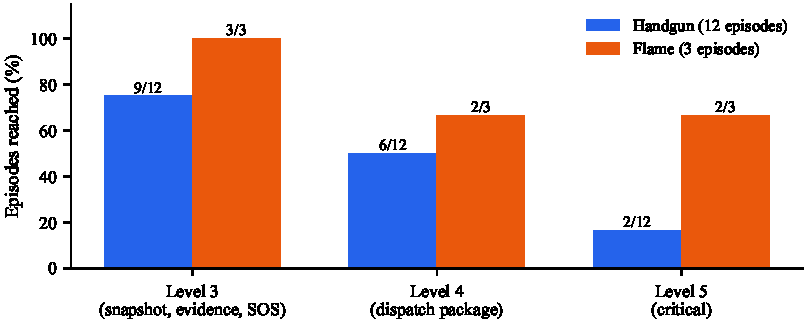
\includegraphics[width=0.85\textwidth]{figures/fig_levels.pdf}
\caption{Episodes reaching each committed level in the replay of the ten videos (tick mode, time-aligned soundtracks)}
\label{fig:levels}
\end{figure}

\begin{table}[htbp]
\caption{Committed-level results (all ten videos, partly in-sample)}
\label{tab:levels-res}
\centering\tablefont
\begin{tabularx}{\textwidth}{|Y|C{2.2cm}|C{2.2cm}|C{2.6cm}|}
\hline\rowhead
\thead{Measure} & \thead{Tick mode, 6\,Hz} & \thead{Tick mode, 2\,Hz} & \thead{Clip mode + fast lane}\\ \hline
Handgun at Level 3 / 4 / 5 & 9/12, 6/12, 2/12 & 9/12 at L3 & 9/12, 6/12, 5/12\\ \hline
Flame at Level 3 / 4 / 5 & 3/3, 2/3, 2/3 & 3/3 at L3 & 3/3, --, 2/3\\ \hline
Robbery / assault at Level 3 & 0/1 / 0/2 & 0/1 / 0/2 & 0/1 / 0/2\\ \hline
False onsets at Level 3 and above (3.7 normal minutes) & 0 & 0 & 0\\ \hline
Upper 95\,\% bound on false Level~3 onsets & 60 per hour & 60 per hour & 60 per hour\\ \hline
Frame AUROC of the scene model, weapon / fire & 0.93 / 0.999 & -- & --\\ \hline
\end{tabularx}
\end{table}

These numbers are encouraging but not a validation: seven of the ten videos were used in training, and 3.7 minutes of normal footage can only bound the false-alarm rate at 60 per hour, far above what a home needs. Two release gates measured on this data fail: G2 (handgun episodes confirmed within 2\,s: 8 of 12) and G4 (onset to Level~3 at the 95th percentile: 4.0\,s against 2\,s).

\subsection{Detector heads retrained on fifteen videos}
The weapon and fire heads were retrained from the v4 heads on all 977 frames (fifteen videos, 180 boxes) with 2000 public images mixed back in, so that the public classes are not forgotten. The weapon head gained knife and long-gun classes. Each head had to pass bars fixed before training:
\begin{itemize}
\item no rise in false alarms on the held-out normal frames of the validation and test videos;
\item validation weapon AUROC not lower by more than 0.02 (fire: not lower);
\item public pistol (fire) AP50 not lower.
\end{itemize}
Both passed (\tabref{tab:v5heads}). On the held-out validation videos the weapon head's frame AUROC rose from 0.748 to 0.871 and the fire head's from 0.587 to 0.964, with no new false alarms. On the public test sets, which the v4 heads had forgotten, pistol AP50 went from 0.007 to 0.699, and the new knife class reached 0.717.

In the replay of all fifteen videos, 11 of 14 weapon episodes reach Level~3 instead of 9: the new handgun and knife scenes now raise an assistance request. The false Level~3 onset count is unchanged at 1 in 4.9 minutes of normal footage. Two results did not improve:
\begin{itemize}
\item the two flames that reached Level~5 now stop at Level~4;
\item the small aerosol flame of \code{vid04} still scores below the fire head's vote.
\end{itemize}
The five new videos are in the training split, so their replay is in-sample.

The scene classifier was not retrained in this step. Measured on the five new videos it recognises the new scenes poorly: accuracy 0.43, macro-F1 0.16, 1 of 47 weapon frames. It raised no false weapon or fire alarm on their 90 normal frames.

\begin{table}[htbp]
\caption{v4 and v5 detector heads (held-out validation: gun, vid04; replay: all fifteen videos, tick mode at 6\,Hz with their soundtracks, partly in-sample)}
\label{tab:v5heads}
\centering\tablefont
\begin{tabularx}{\textwidth}{|Y|C{3.0cm}|C{3.0cm}|}
\hline\rowhead
\thead{Measure} & \thead{v4 heads} & \thead{v5 heads}\\ \hline
Validation frame AUROC, weapon / fire & 0.748 / 0.587 & \textbf{0.871 / 0.964}\\ \hline
False alarms on held-out normal frames at 0.25 (validation / test), weapon & 0.000 / 0.015 & 0.000 / 0.015\\ \hline
Public test AP50: pistol / knife / fire & 0.007 / -- / 0.000 & \textbf{0.699 / 0.717 / 0.487}\\ \hline
Weapon episodes at Level 3 / 4 / 5 & 9/14, 6/14, 2/14 & \textbf{11/14}, 6/14, 2/14\\ \hline
Flame episodes at Level 3 / 4 / 5 & 3/3, 2/3, 2/3 & 3/3, 2/3, 0/3\\ \hline
False onsets at Level 3 (4.9 normal minutes) & 1 & 1\\ \hline
\end{tabularx}
\end{table}

\subsection{Real-time performance}
\figref{fig:liveloop} shows the live loop on the laptop before and after the M2 repair, measured with \code{tools/bench\_live.py} on a video with four faces. Separating capture, inference and preview, turning off the ONNX Runtime spin-wait and moving face recognition to its own thread raised the preview from 0.6 to 29.7\,fps and the AI rate from 0.32 to 5.6 decisions per second (tick p50 168\,ms, frame age p50 198\,ms).

\begin{figure}[htbp]
\centering
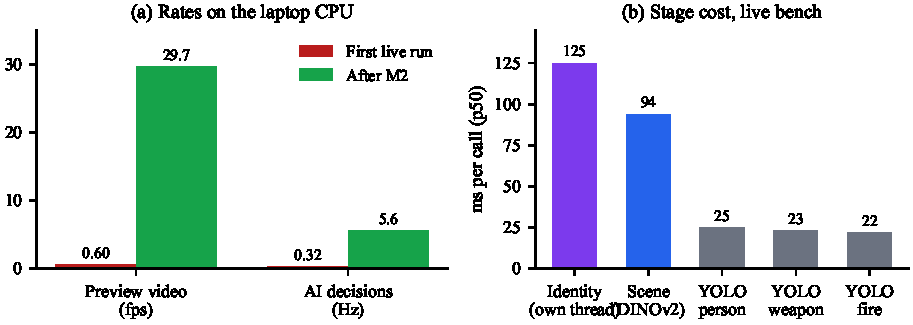
\includegraphics[width=\textwidth]{figures/fig_live_loop.pdf}
\caption{Live loop on the laptop CPU: (a) preview and AI rates before and after M2; (b) cost of each stage}
\label{fig:liveloop}
\end{figure}

On the Raspberry~Pi~5 the same models must share four cores. \figref{fig:piclip} shows the clip engine measured on the Pi with the held-out handgun clip as a 30\,fps camera. At 640\,px the object stage alone takes 5.6\,s and three clips in four are dropped; at 320\,px the clip takes 3.9\,s, every other clip is analysed and decisions are about 4\,s old, with the same Level~3 recall on the replay (9/9 handgun, 3/3 fire on the nine training and validation videos) and one Level~4 handgun episode fewer. The shipped profile is therefore 320\,px with two scene frames; the fast lane (about 3.5 passes per second, 35--39\,ms per head at 320\,px) provides the quick Level~3 path. The 1.6\,s budget is not yet met: the DINOv2 stage alone takes about 1.2\,s per frame on the Pi, which is why a Hailo NPU or an NCNN build is the planned next step.

\begin{figure}[htbp]
\centering
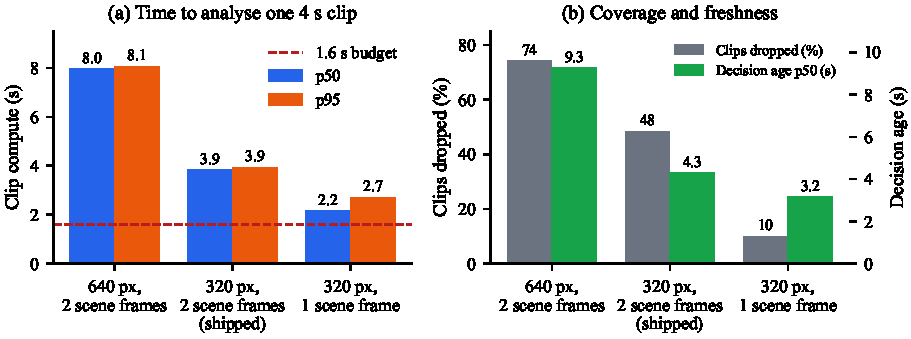
\includegraphics[width=\textwidth]{figures/fig_pi_clip.pdf}
\caption{Clip engine on the Raspberry~Pi~5: (a) time to analyse one 4\,s clip; (b) share of clips dropped and age of decisions}
\label{fig:piclip}
\end{figure}

\subsection{Slim models for the Pi (a rejected hypothesis)}
To make the scene stage fit the Pi, MobileNetV3-L and EfficientNet-B0 heads were trained under a protocol fixed in advance (\figref{fig:slim}). They are 25--40 times faster (2.4 and 4.3\,ms in ONNX Runtime) but reach LOVO macro-F1 of only 0.229 and 0.211 against 0.440 for DINOv2, below the pre-registered bar of 0.396, and neither recognises fire in a video it has not seen. Distillation from DINOv2 did not help (0.211--0.224): the cross-video generalisation of DINOv2 lies in its self-supervised features, which an ImageNet CNN does not have. DINOv2 stayed in the product.

\begin{figure}[htbp]
\centering
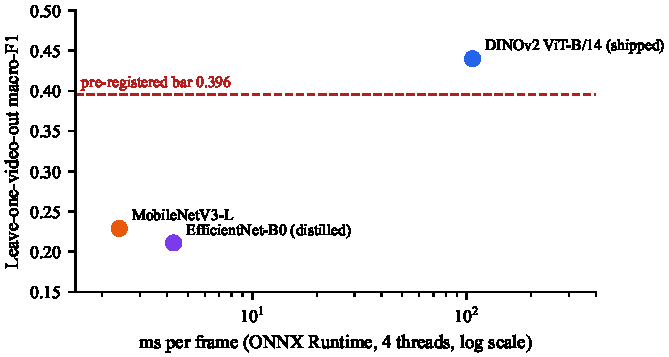
\includegraphics[width=0.72\textwidth]{figures/fig_slim.pdf}
\caption{Accuracy against speed of the scene classifiers (leave-one-video-out)}
\label{fig:slim}
\end{figure}

\subsection{Body re-identification}
\figref{fig:reid} shows the evaluation of body matching on ByteTrack tracks of the nine training and validation videos (4524 same-person pairs, 2498 different-people pairs).
\begin{itemize}
\item \textbf{Same weights as the prototype.} The earlier IntrusionSentry prototype used OSNet x1\_0 with ImageNet weights. These separate people better than colour histograms (AUROC 0.83 against 0.73).
\item \textbf{Re-identification-trained weights.} OSNet x1\_0 and OSNet-AIN x1\_0, both trained for re-identification on MSMT17, do better still (0.92 and 0.93). OSNet-AIN was chosen by a rule fixed before the comparison: the most same-person cases at a bar that accepts at most 0.05\,\% of different people.
\item \textbf{Speed.} These checkpoints contain denormal weights, which made CPU inference 6--17 times slower. Zeroing them brought OSNet-AIN to 10.3\,ms per crop with unchanged features.
\end{itemize}
With the five November videos (fourteen videos; 1500 same-person and 25,408 different-people cases of the identity rule), the bar moved from 0.86 to 0.87. The rule, 20 looks and two checks in a row, reaches AUROC 0.97 and accepts 30\,\% of same-person cases and 0.020\,\% of different people.

The prototype's cosine bar of 0.50 would have accepted 97.2\,\% of different people on the ImageNet features and 50\,\% on the shipped ones. At SENTRIX's bar a wrong match is rare, and it can at most hide a Level~2 notice at home.

\begin{figure}[htbp]
\centering
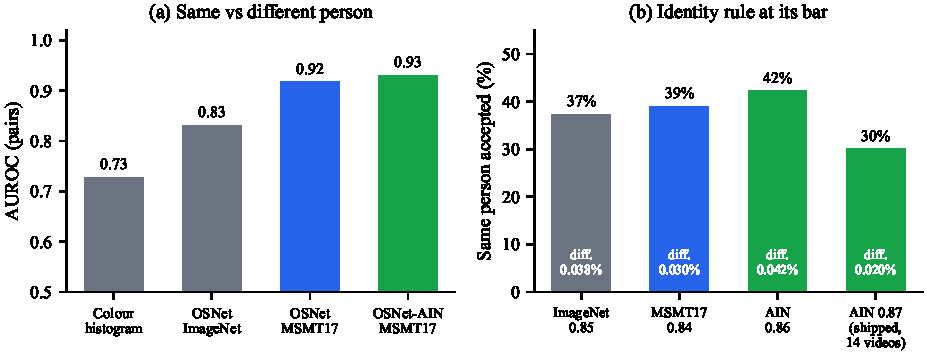
\includegraphics[width=\textwidth]{figures/fig_reid.pdf}
\caption{Body re-identification: (a) separation of same and different people with four body models (nine videos); (b) the identity rule at each model's bar, and the shipped OSNet-AIN bar on fourteen videos}
\label{fig:reid}
\end{figure}

\subsection{Calibration in the demonstration room}
In about ten hours after the Pi was installed in the demo room, the scene classifier alone raised 16 weapon Level~3 alarms (the weapon detector confirmed none), and later two fire Level~3 alarms, with no weapon or flame present. The Pi's own logs (8077 clips for weapon, 5435 scored clips for fire) show why (\figref{fig:room}): in this room the classifier's p(weapon) has a median of 0.19 but a 99.9th percentile of 0.65 and a maximum of 0.742, above the 0.50 floor; p(fire) peaks at 0.646 against a 0.45 floor. Per-room thresholds of 0.75 (weapon) and 0.70 (fire) remove every one of these false alarms. The cost is stated openly: a small flame that the classifier scores below 0.70 (the held-out vid04 peaks at 0.636 in clip mode) no longer reaches Level~3 from the classifier alone and needs the fire detector; the replica-gun and replica-flame tests in that room are part of the remaining work.

\paragraph{Calibration from the device's own log.} Setting those thresholds meant reading the Pi's log by hand, and every new room or new model would need it again. A tool now does it by a rule fixed in advance (\code{tools/calibrate\_room.py}, decision D23). It reads the device's own event log for a period the team asserts was quiet, and replays the device's confirmation rule at every possible threshold. On the Pi that rule is two keyframes per clip, with a weapon keyframe counting only if a person was seen in the last 2\,s; the replay rebuilds that gate from the logged person boxes. It then proposes
\begin{equation}
\theta_c = \max\big(\text{floor}_c,\ \hat{c}_c + 0.10,\ \hat{s}_c + 0.01\big),
\label{eq:calib}
\end{equation}
rounded up to 0.01, where $\hat{c}_c$ is the highest value at which a quiet clip would still have been confirmed and $\hat{s}_c$ the highest single score. The tool also checks itself: wherever the device logged its own decision, the replay at the device's threshold must reach the same one.

On the Pi it was run over SSH and read the logs without changing anything on the device. \tabref{tab:calib} shows the results:
\begin{itemize}
\item \textbf{Check:} the replay matched the device's own decision on all 8,956 logged clips.
\item \textbf{Hand thresholds reproduced:} on the data each hand threshold was set from, the rule gives weapon 0.76 (hand: 0.75) and fire 0.69 (hand: 0.70).
\item \textbf{Whole log:} from 23 October to 19 November the scene model scored 9,092 clips (5.1\,h). The thresholds in force gave no confirmation at all, against 45 weapon and 4 fire onsets at the floors. The 95\,\% upper bound is 0.59 false onsets per hour.
\end{itemize}

The margins were thinner than the rule asks for. One keyframe reached p(weapon) 0.760, above the 0.75 threshold, and a fire confirmation reached 0.650, 0.05 under it. On 19 November the owner therefore approved the proposal, weapon 0.78 and fire 0.75, and it is now in force on the Pi (\figref{fig:room}).

The calibration file records the scene model it was made for. If another model loads, the device keeps the thresholds but flags them as stale, so a retrained model is followed by a new calibration.

The cost is the same as before, one step higher: a replica gun or flame scored between the old and new thresholds no longer reaches Level~3 from the scene model alone. The replica tests in that room, which the tool can replay with \code{--check}, are still to do.

\begin{table}[htbp]
\caption{Room calibration of the demonstration Pi from its own log (clip mode, v4 scene model)}
\label{tab:calib}
\centering\tablefont
\begin{tabularx}{\textwidth}{|Y|C{3.2cm}|C{3.2cm}|}
\hline\rowhead
\thead{Measure} & \thead{Weapon} & \thead{Fire}\\ \hline
Data each hand threshold was set from: scored time & 1.96\,h & 2.40\,h\\ \hline
\quad highest single score / confirming value & 0.742 / 0.590 & 0.646 / 0.587\\ \hline
\quad threshold set by hand / by \eqnref{eq:calib} & 0.75 / 0.76 & 0.70 / 0.69\\ \hline
Whole log (23 Oct -- 19 Nov, 5.1\,h scored): median / p99 / max score & 0.190 / 0.546 / 0.760 & 0.079 / 0.236 / 0.716\\ \hline
\quad onsets at the floor / at the hand threshold & 45 at 0.50 / 0 at 0.75 & 4 at 0.45 / 0 at 0.70\\ \hline
\quad proposed and in force since 19 Nov & \textbf{0.78} & \textbf{0.75}\\ \hline
Replay agrees with the device's own decision & \multicolumn{2}{c|}{8,956 of 8,956 clips}\\ \hline
\end{tabularx}
\end{table}

\begin{figure}[htbp]
\centering
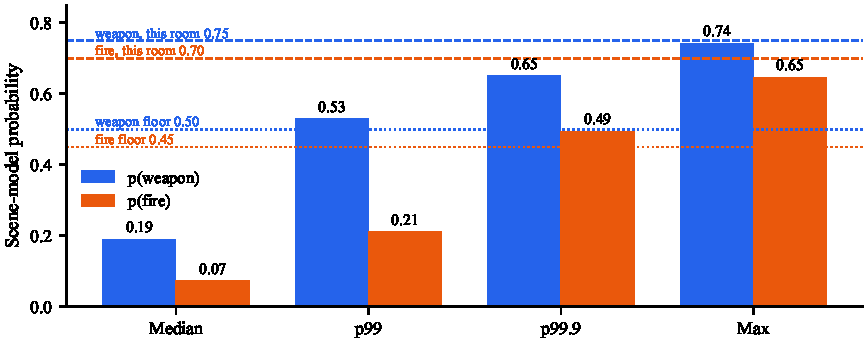
\includegraphics[width=0.92\textwidth]{figures/fig_room_scores.pdf}
\caption{Scene-classifier probabilities in the demo room with no threat present (whole log, 5.1\,h scored), with the default floors and the calibrated room thresholds}
\label{fig:room}
\end{figure}

\subsection{Comparison with related work}
\tabref{tab:sota} compares SENTRIX's components and system-level behaviour with published work. Component scores are not directly comparable---the published numbers come from large public benchmarks and SENTRIX's from two rooms---so the table is read for what each approach measures and where SENTRIX differs.

\begin{table}[htbp]
\caption{Comparison with related state-of-the-art work}
\label{tab:sota}
\centering\tablefont
\begin{tabularx}{\textwidth}{|L{2.4cm}|Y|Y|}
\hline\rowhead
\thead{Aspect} & \thead{Published work} & \thead{SENTRIX}\\ \hline
Handgun alarm & Faster R-CNN alarm after five successive detections fired correctly in 27 of 30 test scenes \cite{olmos2018handgun} & YOLO11n + DINOv2 with 2-of-3 confirmation and a person gate: 9 of 12 episodes at Level~3, 0 false onsets in 3.7 normal minutes (11 of 14 on fifteen videos with the v5 heads); room thresholds calibrated from the device's own logs\\ \hline
Violence & Flow-gated 3D-CNN: 87.25\,\% test accuracy on RWF-2000 \cite{cheng2021rwf}; audio-visual fusion improves XD-Violence \cite{wu2020xdviolence} & ResNet-18 on RWF-2000: 0.832 macro-F1 on a contaminated split; in the product a fight needs video \emph{and} aligned aggression audio, with a banter rule\\ \hline
Audio tagging & PANNs: best model 0.439 mAP on AudioSet \cite{kong2020panns} & PANNs CNN10 at 40\,ms per 4\,s window on a CPU, 527 labels mapped to 7 cues, votes only when time-aligned\\ \hline
Re-identification & OSNet: state of the art on six re-ID datasets with re-ID training \cite{zhou2019osnet} & OSNet-AIN trained on MSMT17 tied to an access decision: AUROC 0.97, 0.020\,\% false accepts at the shipped bar (fourteen videos)\\ \hline
Evaluation & Frame accuracy, mAP or AUROC on curated test sets & Committed-level episodes, false onsets per hour with exact Poisson bounds, onset latency; pre-registered model selection\\ \hline
Alert flow & Detection only, or direct alerting & Owner-approved request, PIN-protected false alarms, duress PIN, safety defaults, ``unanswered'' never ``safe''\\ \hline
Deployment & GPU servers or cloud analysis \cite{shi2016edge} & All inference on a Raspberry~Pi~5; video, faces and evidence stay at home\\ \hline
Recent detectors (2024--2026) & NMS-free YOLOv10s and YOLO26s: 125--130\,ms per frame on a Jetson Nano \cite{fierrosilva2026yolo26weapon}; a review of 101 weapon papers finds little real-world validation \cite{murugan2025weaponreview} & YOLO11n heads at 320\,px take 35--39\,ms per head on the Pi~5 CPU and are judged by committed level in real rooms; YOLO26 is next\\ \hline
VLM and LLM anomaly detection & VadCLIP: 84.51\,\% AP on XD-Violence \cite{wu2024vadclip}; LAVAD: 80.28\,\% AUC on UCF-Crime without training \cite{zanella2024lavad}; MLLMs still limited on smart-home video \cite{zhao2025smarthomebench} & Supervised detectors and published rules on the device; no model's verdict replaces the owner's\\ \hline
Audio-visual fusion (2025) & Align-then-fuse: 86.07\,\% AP on XD-Violence \cite{jin2025aligning} & Time-stamped windows vote only when aligned; banter holds a fight at Level~2\\ \hline
Industry practice & Cloud face recognition in doorbells (2025) \cite{perez2025ringfaces}; police dispatch only with audio, video or witness evidence (2024) \cite{seattle2024alarm} & Faces stay on the device; every request carries a snapshot and a timeline\\ \hline
\end{tabularx}
\end{table}

\section{Inferences Drawn}
\begin{enumerate}
\item \textbf{The decision rules matter more than any single model.} The same models produced 9 Level~3 onsets in 18 minutes or none, depending only on confirmation and corroboration rules.
\item \textbf{Training on one's own footage beats bigger public datasets.} A self-supervised backbone fine-tuned on 765 frames of the target setting outperformed models trained on thousands of public images on every held-out measure except the one class (stick) that the custom data barely contained.
\item \textbf{A new room is a new distribution.} Thresholds valid on the training rooms produced false alarms in the demo room until the room's own logs set them; per-room calibration (now a tool that replays the device's own rule) and deployment-room recordings are part of installing the product, not an afterthought.
\item \textbf{Measuring what the user experiences changes the conclusions.} Per-frame accuracy looked acceptable while the product was unusable; committed-level metrics with confidence bounds showed both the progress and how little normal footage had been seen.
\item \textbf{The Pi can run the whole product, but not yet within the latency target.} With the clip engine and ONNX it analyses every other clip and decides within about 4\,s; the transformer backbone is the bottleneck.
\item \textbf{Safety must be designed into the alert flow.} Silence is not safety, a PIN prevents an intruder from cancelling, and a duress path protects a coerced owner; all of these are testable logic, and the tests found real defects.
\end{enumerate}

\section{Validation of Objectives}
\label{sec:validation}

\begin{table}[H]
\caption{Validation of the approved objectives}
\label{tab:validation}
\centering\tablefont
\begin{tabularx}{\textwidth}{|L{2.4cm}|Y|L{1.6cm}|}
\hline\rowhead
\thead{Objective} & \thead{What was built and the evidence} & \thead{Status}\\ \hline
O1 Multimodal AI pipeline & Weapon (handgun, knife, long gun) and fire detection (YOLO11n), scene and fight classification (DINOv2), faces (InsightFace), bodies (OSNet-AIN), sound (PANNs CNN10), in tick and clip pipelines; handgun 9/12 and flame 3/3 at Level~3 on replay (weapon 11/14 on fifteen videos); 29.7\,fps preview and 5.6\,Hz AI on a laptop; 3.9\,s per clip on the Pi & Achieved; Pi latency target open\\ \hline
O2 Fusion into a TCI & The learned XGBoost fusion of the mid-semester version was retired: it had been fitted to synthetic labels with the meaning of identity inverted and ranked threats worse than its own inputs. It was replaced by transparent, time-aligned evidence rules that produce the same 0--1 TCI and five levels, with every decision re-derivable from the log; live false onsets at Level~3+ fell from 9 to 0 & Achieved with a changed method\\ \hline
O3 Tamper-evident evidence & AES-256-GCM bundles with HKDF keys, SHA-256 digests and an HMAC-signed hash-chained manifest; pre-roll clips in clip mode; a verifier checks every digest and the signed chain & Achieved\\ \hline
O4 Physical edge unit & Raspberry~Pi~5 unit with Camera Module 3, USB microphone, PIR, door and mains inputs, LEDs and a siren relay; bill of materials about Rs.\,40,500 including tools; parametric enclosure; running in the demo room as a systemd service. The ESP32 and DHT22 design of the proposal was replaced by the Pi~5 for camera and audio quality & Achieved (budget revised)\\ \hline
O5 Command console and alerting & React device screen and administration pages, React Portal with onboarding, live view through the tunnel, owner-approved SOS over Portal, device screen, Telegram, e-mail and SMS, the SENTRIX Desk and the admin console; 22 of 23 browser tests pass & Achieved; one UI defect open\\ \hline
\end{tabularx}
\end{table}
